\chapter{Introducción}
\label{int}

\section{Contexto general de esta tesis}
\label{int:s:contexto}

    La teledetección o sensoramiento remoto del entorno terrestre fue cobrando creciente importancia desde su nacimiento (hace aproximadamente 50 años) con el avance de la tecnología espacial; la creciente disponibilidad y diversidad de instrumentos midiendo tanto desde el espacio como \textit{in situ}; la gratuidad y el creciente volumen de los datos adquiridos por dichos instrumentos para su uso científico; el constante avance en el grado de sofisticación de los algoritmos utilizados para extraer información biogeofísica de las imágenes, entre otros. Su aplicación en la evaluación de recursos naturales y el monitoreo de factores ambientales se inició en 1972 con el lanzamiento de la plataforma Landsat 1 \cite{landsat1}, un sistema de prueba de concepto cuyos resultados positivos fomentaron de manera vertiginosa el desarrollo de la tecnología espacial, con fines de monitorear el entorno terrestre. En 1978 cesaron las conexiones con dicha plataforma, pero a su vez fue el año en que se lanzó la plataforma Nimbus 7, la primera misión que portaba un sensor con fines específicos a la teledetección de cuerpos de agua en el rango visible: el \textit{Coastal Zone Color Scanner} (CZCS).
    
    A pesar de que fue originalmente una prueba de concepto destinada a durar un año, el CZCS continuó generando una serie temporal de datos muy valiosos hasta 1986, que permitieron por primera vez observar sinópticamente la distribución espacial y temporal de la concentración de clorofila (Chavez 1995, \cite{chavez1995}) - sustancia utilizada como \textit{proxy} de la biomasa fitoplanctónica - en distintas regiones del mundo y también ha permitido estimar la producción primaria a escala global. Diez años pasaron antes de que otros sensores destinados a proveer datos de color del mar orbitasen nuevamente alrededor de la Tierra. En particular, el SeaWiFS (\textit{Sea-viewing Wide Field-of-view Sensor}) - lanzado en 1997 a bordo del satélite SeaStar de la NASA - fue el que interrumpió esta década sin disponibilidad de sensores y produjo datos hasta 2010 (Figura \ref{int:sensor_timelines}). Algunos de los sensores posteriores más destacados fueron los MODIS (\textit{Moderate-resolution Imaging Spectroadiometer}) a bordo de los satélites Terra y Aqua (lanzados en 1999 y 2002 resp. y actualmente en funcionamiento) y el MERIS (\textit{MEdium Resolution Imaging Spectrometer}) a bordo del satélite Envisat de la Agencia Espacial Europea (ESA) que fue lanzado en 2002 y dejó de ser operacional en 2012. Otros sensores destinados al sensoramiento remoto de cuerpos de agua en el rango óptico - de aquí en más denominado \textit{color del mar} - fueron lanzados más recientemente, incluyendo el OCM-2 (\textit{Indian Ocean Colour Monitor}), el GOCI (\textit{Korean Geostationary Ocean Color Imager}, el primer sensor geoestacionario destinado a color del mar), el VIIRS (\textit{Visible Infrared Imager Radiometer Suite }) y los sensores OLCI (\textit{Ocean and Land Color Instrument}) A y B a bordo de las plataformas Sentinel-3 A y B. Nuevos sensores de color del mar están planeados dentro de la siguiente década por varias agencias espaciales, entre ellas la misión PACE (Pre-Aerosol, Clouds and ocean Ecosystem) que será lanzada por la NASA y la misión argentino-brasileña SABIA-Mar (Satélite Argentino-Brasileño para la Información del Mar). El Cuadro \ref{int:tab:sensores} muestra un listado de los sensores considerados en la presente tesis, junto con sus principales características: ciclo de revisita, resolución espacial, rango espectral y número de bandas.

    \begin{figure}
    \centering
    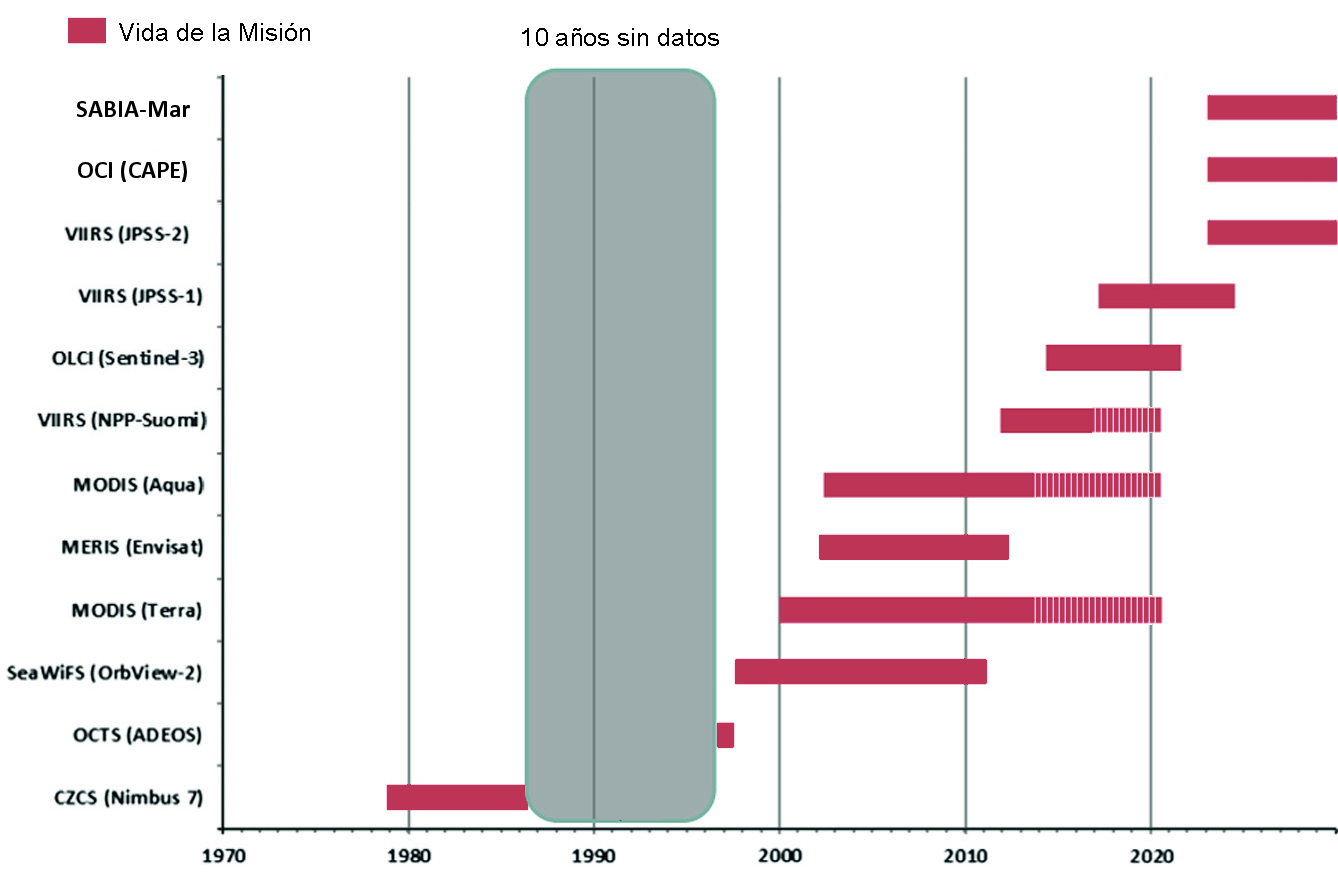
\includegraphics[width=\textwidth]{int/figures/sensor_timelines.png}
    \caption[Línea de tiempo con las principales misiones de color del mar en el período 1978-2030.]{Línea de tiempo con las principales misiones de color del mar en el período 1978-2030. Las barras indican el tiempo de vida útil y las barras rayadas verticalmente indican la extensión de la vida útil más allá del pronóstico inicial.}
    \label{int:sensor_timelines}
    \end{figure}

    \begin{table}
        \small
        \caption[Sensores utilizados en la presente tesis con sus características principales.]{Sensores utilizados en la presente tesis con sus características principales: ciclo de revisita, resolución espacial, rango espectral y número de bandas.}
        \begin{tabular}{|l|l|l|l|l|}
        \hline
        \textbf{Plataforma/Sensor}   & \textbf{\begin{tabular}[c]{@{}l@{}}Ciclo de revisita\\ {[}días{]}\end{tabular}} & \textbf{\begin{tabular}[c]{@{}l@{}}Resolución\\ espacial {[}m{]}\end{tabular}} & \textbf{\begin{tabular}[c]{@{}l@{}}Rango\\ espectral\\ {[}nm{]}\end{tabular}} & \textbf{\begin{tabular}[c]{@{}l@{}}Número\\ de bandas\end{tabular}} \\ \hline
        \textbf{Aqua-Terra/MODIS}    & 1    & 250/1000 & 400-2130 & 16 \\ \hline
        \textbf{LandSat-8/OLI}       & 16   & 30       & 433-2300 & 7  \\ \hline
        \textbf{SABIA-MAR/VNIR-SWIR} & 2    & 200      & 412-1640 & 16 \\ \hline
        \textbf{Sentinel-2/MSI}      & 5    & 10       & 443-2190 & 13 \\ \hline
        \textbf{Sentinel-3/OLCI}     & 2    & 300      & 400-1040 & 21 \\ \hline
        \textbf{Suomi-NPP/VIIRS}     & 1    & 750      & 410-2257 & 10 \\ \hline
        \end{tabular}
        \label{int:tab:sensores}
    \end{table}

    La ciencia del color del mar, posible gracias a la operatividad de estos sensores y a la comunidad científica que la desarrolla, ha demostrado su capacidad de proveer información sinóptica de las propiedades ópticas y biogeoquímicas de los océanos, \cite{tilstone2003b}\cite{blondeau2014}\cite{odermatt2016}. Esta se basa en la determinación de la radiancia espectral que proviene de la superficie del agua y ha demostrado ser una técnica muy fructífera ya que permite estimar la concentración de variables biogeofísicas como la concentración de clorofila-a, de material particulado en suspensión (\textit{Suspended Particulate Matter}, SPM) y la turbidez en áreas muy extensas y de manera periódica, resultando así una herramienta complementaria a las costosas mediciones de campo. Los datos satelitales del color del mar son utilizados para estudiar global y regionalmente la biosfera oceánica, su cambio en el tiempo y cómo se relaciona este cambio con las actividades antropogénicas. Los sensores satelitales de color del mar permiten detectar y cuantificar tendencias globales en las propiedades biogeoquímicas, tanto estacionales como en escalas temporales de décadas. Asimismo, constituyen una herramienta fundamental para la estimación de la producción primaria del \textit{fitoplancton} (organismos acuáticos autótrofos que tienen capacidad fotosintética y que viven dispersos en el agua) y que permite, junto con otras variables, delimitar zonas marinas de protección; como así también identificar potenciales zonas de pesca contribuyendo a un manejo sustentable de los recursos pesqueros, \cite{ioccg2008}.
    
    Las series temporales de propiedades de color del mar tienen aplicación en el estudio del cambio climático global \cite{dutkiewicz2019} - de hecho el color del mar ha sido clasificado como Variable Climática Esencial por el programa GCOS (\textit{Global Climate Observing System}) de la Organización Meteorológica Mundial (\textit{World Meteorological Organization}, WMO, \cite{wmoweb}). Mediante el conocimiento sobre la intensidad luminosa y la eficiencia fotosintética - obtenida mediante color del mar - es posible producir mapas de Producción Primaria Neta (Net Primary Production, NPP) sobre los océanos, es decir, indicadores de cuánto dióxido de carbono son capaces de fijar los organismos autótrofos y mixótrofos presentes en el agua, \cite{carr2006}. De esta forma, los datos del color del mar resultan esenciales en la determinación del balance global de dióxido de carbono, permitiendo mejorar el entendimiento de la tasa neta - actualmente positiva - de inyección de este gas de efecto invernadero en la atmósfera y los océanos.
    
    A su vez, los datos de color del mar junto con datos meteorológicos y de campo han sido utilizados para la detección temprana de floraciones algales nocivas, \cite{stumpf2003b}, a veces popularmente conocidas como \textit{mareas rojas}, las cuales impactan fuertemente en las actividades pesqueras. También han sido empleados para la detección y el análisis de la distribución espacial y temporal de zonas de máxima turbidez en diferentes ríos como el Río Girondo en Francia, \cite{doxaran2006}, o el Río de la Plata \cite{framinan1996}. En este último caso, la zona de máxima turbidez es un área de importancia económica y ecológica ya que es una zona de alta concentración de \textit{plancton} \cite{acha2004} y es el área principal de desove y de cría para muchas especies del estuario que se explotan comercialmente y sostienen las pesquerías costeras de Argentina y Uruguay, \cite{macchi1996}\cite{acha1999}\cite{jaureguizar2003}.
    
% ;  La complejidad adicional que supone la corrección atmosférica en aguas ópticamente complejas dio lugar a una variedad de alternativas, muchas de las cuales resultaron originalmente adecuadas en entornos de aguas moderadamente complejas \cite{stumpf2003}\cite{bailey2010}\cite{ruddick2000}, pero no en aguas extremadamente complejas como el Estuario del Río de la Plata - es decir, nuestra región de interés.
 
    Uno de los problemas más importantes a los que se enfrentan los científicos a la hora de dar uso a las imágenes obtenidas por los sensores de color del mar es la no transparencia de la atmósfera en las longitudes de onda de interés, por lo que es necesario el diseño de un algoritmo que remueva el efecto producido por la atmósfera en el flujo radiativo que, tras atravesar la atmósfera e interactuar con el entorno terrestre, arriba al sensor. Dicha metodología se denomina \textit{corrección atmosférica} (CA) y la primera en ser aplicada operativamente a imágenes ópticas fue diseñada por Howard Gordon para el pionero sensor CZCS, \cite{gordon1978}\cite{gordon1980}\cite{viollier1980}\cite{gordon1981}\cite{gordon1987}\cite{gordon1988}. Paradójicamente, el principio de funcionamiento de la CA radicaba en supuestos que se cumplían únicamente en aguas oligotróficas del océano abierto, siendo que el objetivo original de la puesta en órbita del CZCS era el monitoreo de aguas costeras, tal como su sigla lo indica. La no validez de dicho supuesto en aguas turbias se traducía en una mala estimación de las reflectancias del agua y, consecuentemente, en bajas concentraciones de clorofila-a, \cite{chavez1995}, un pigmento fotoactivo presente en la totalidad de los organismos fotosintéticos.

    Lo expuesto resalta que la precisión de las correcciones atmosféricas es fundamental en el área de color del mar dado que de ellas depende la capacidad de obtener la reflectancia medida justo sobre la superficie del agua, $\rho_{w}$, magnitud de base para los algoritmos bio-ópticos que la utilizan como entrada para estimar la concentración de diferentes propiedades ópticas o sustancias de interés. En general, del total de la radiación que llega al sensor, sólo una pequeña proporción de la misma corresponde a la señal que proviene del agua. Esta puede ser menor al 10\% en la región azul del espectro y mucho menor en las bandas infrarrojas, \cite{gordon1999}. Por lo tanto la aplicación de una corrección atmosférica sumamente precisa es fundamental para poder estimar plausiblemente el tipo y cantidad de sustancias presentes en el agua.
    
    La corrección diseñada e implementada por Howard Gordon para CZCS suponía que el agua absorbe toda la luz en la región del rojo e infrarrojo cercano (Near Infra-Red, NIR) del espectro electromagnético (supuesto de \textit{agua negra} o \textit{píxel negro}) permitiendo estimar la contribución de la atmósfera en esta región del espectro, extrapolarla a la región del visible ($400-600$ nm) y determinar así la componente que proviene de la capa superficial del agua y que contiene la información deseada (\S \ref{int:s:ACblackPixelNIR}). Sin embargo, en aguas altamente productivas o turbias, la alta concentración de partículas en suspensión incrementa mucho la dispersión de la energía en el NIR, por lo que la reflectancia del agua en esta región del espectro deja de ser nula - es decir que el supuesto de agua negra deja de ser válido, \cite{siegel2000}\cite{stumpf2003}. Asumir que la reflectancia del agua en el NIR es cero en aguas productivas o turbias lleva a una sobreestimación de la contribución de los aerosoles y subsecuentemente a una subestimación de la reflectancia del agua en la región visible del espectro, \cite{bailey2010}. Varios algoritmos han sido desarrollados con hipótesis alternativas o incluyendo esquemas que tienen en cuenta la contribución del agua en la señal total que llega al sensor \cite{stumpf2003}\cite{bailey2010}\cite{moore2011}\cite{ruddick2000}\cite{ruddick2006}, \S \ref{int:s:ACiterNIR},\ref{int:s:ACmumm}. Estos últimos algoritmos estiman o modelan la señal que proviene del agua en el NIR (supuesto de \textit{píxel brillante}) para luego restársela a la señal total y así poder aplicar la CA tradicional, es decir, utilizando el supuesto de agua negra. Otra estrategia propuesta ha sido utilizar bandas en longitudes de onda más largas en el infrarrojo de onda corta (Short Wave Infrared, SWIR, $1000-3000$ nm), donde la absorción del agua es tan alta que puede asumirse que la componente que proviene del agua sí es despreciable en esta región del espectro, \S \ref{int:s:ACswir}. Esto es equivalente a decir que dicha estrategia se respalda en el supuesto de agua negra, pero en el SWIR en vez del NIR. La problemática fundamental de dicha estrategia es que muchos de los sensores de color del mar carecen de dichas bandas o bien las poseen pero sin la suficiente relación señal ruido (\textit{Signal-to-Noise Ratio}, SNR), \cite{wang2018}.

    El color del mar es una variable fundamental para todas aquellas naciones con extensas líneas de costa con interés en monitorear y explotar su litoral marítimo, como es el caso de la República Argentina, donde recientemente nació la Iniciativa Pampa Azul \cite{pampaazul}, cuyo objetivo estriba en la imperante necesidad del país de continuar desarrollando una explotación eficiente y sustentable de sus recursos pesqueros. En el marco de la iniciativa, una de las regiones reconocidas de interés es el sistema fluvio-marino del Río de la Plata, cuyas aguas son críticas para las pesquerías costeras de especies como lenguado, pescadilla, gatuzo, raya, pez palo, corvina negra, saraca, pescadilla real y besugo, \cite{pampaazulrdp}. Por otro lado, la Comisión Nacional de Actividades Espaciales (CONAE) en conjunto con la Agencia Espacial Brasileña (AEB) y el Instituto Nacional de Investigación Espacial de Brasil (INPE) se encuentran actualmente desarrollando la misión SABIA-Mar, \cite{conaeSMar}\cite{invap}, cuyo principal objetivo es proveer información y productos para el estudio de los ecosistemas marinos, el ciclo del carbono, la cartografía de costas y hábitats marinos, peligros en el litoral marino, aguas continentales y las actividades pesqueras, \cite{conaeSMar}. Los sensores ópticos del SABIA-Mar tendrán bandas espectrales compatibles con los sensores SeaWiFS, MODIS, VIIRS, MERIS y OLCI. A su vez, SABIA-Mar contará con una resolución de 200 m en las áreas de interés específico que constituyen las zonas costeras y marítimas de Argentina y Brasil, como así también las aguas continentales de América del Sur, y una resolución de 800 m para estudios regionales y de cobertura global del océano con el fin de mantener una continuidad y compatibilidad con las demás misiones de color. Según se encuentra actualmente planeada la misión, SABIA-Mar contará con las bandas que también posee MODIS para la CA (tanto en el NIR como en el SWIR, a excepción de la banda en 2130 nm) más dos bandas que también han sido incorporadas en el sensor OLCI de la ESA, entre las cuales la banda en 1016 nm (SWIR cercano) ha demostrado ser útil tanto para la corrección atmosférica como para la estimación del SPM en aguas turbias, \cite{gossn2019}\cite{knaeps2012}.

    En este contexto, esta tesis fue concebida con el objetivo general de generar algoritmos alternativos de corrección atmosférica para ser aplicables sobre imágenes de sensores remotos con diferentes características espectrales en las aguas ópticamente complejas del Estuario del Río de la Plata, así como trabajar sobre aplicaciones novedosas del sensoramiento remoto en el visible sobre aguas con características ópticas afines. De esta forma, y en el marco de la Iniciativa Pampa Azul, esta tesis pretende generar un humilde aporte mediante el desarrollo de herramientas que permitan mejorar la comprensión del sistema fluvio-marino del Río de la Plata, de vital importancia económica para los países que lo conforman.
    
    En este capítulo presentaremos los antecedentes y los conceptos teóricos necesarios para un adecuado entendimiento de los capítulos posteriores. Partiremos definiendo brevemente las magnitudes físicas básicas utilizadas en el sensoramiento óptico de color del mar, partiendo del flujo radiante y concluyendo en la reflectancia del agua. Luego, describiremos las diferentes componentes del balance radiativo total que arriba al sensor, para después describir los diferentes procesos que son considerados por las CAs, necesarias para obtener la reflectancia del agua. Haremos particular hincapié en las diferentes estrategias existentes para la correcciones de aerosoles - la etapa más compleja de una CA - donde expondremos tanto el algoritmo estándar de corrección en aguas claras como las múltiples alternativas que surgen para corregir imágnes sobre escenarios de aguas ópticamente complejas. Describiremos a continuación nuestra área de estudio, el Estuario del Río de la Plata. Finalmente, presentaremos los objetivos de la tesis y un breve resumen del contenido de los capítulos posteriores.

\section{Magnitudes radiométricas utilizadas en teledetección}
\label{int:s:radiometricas}

    El sensoramiento remoto o la \textit{teledetección} es una técnica que permite adquirir información mediante el análisis de datos colectados por instrumentos que no están en contacto físico con los objetos investigados. Los sensores remotos, generalmente a bordo de aviones o satélites que orbitan la Tierra, miden la energía o radiación electromagnética (REM) que es reflejada o emitida por los objetos. Dicha radiación es cuantificada a partir de varias magnitudes físicas, entre las cuales están la irradiancia, la radiancia y la reflectancia, definidas a continuación. Se asumirán escenarios con campos de radiación estacionarios, por lo que se omitirá la dependencia del tiempo de las magnitudes presentadas.

	\subsection{Ángulos de observación-iluminación}
	\label{int:s:geometricas}
	
        Previo a introducir las magnitudes radiométricas, es necesario definir la convención usual utilizada en teledetección para determinar las direcciones de incidencia solar y de observación. En la Figura \ref{int:obs_ilum} se esquematiza el sistema sol-sensor en conjunto con los ángulos asociados a la geometría de observación-iluminación.
        
        \begin{figure}
        \centering
        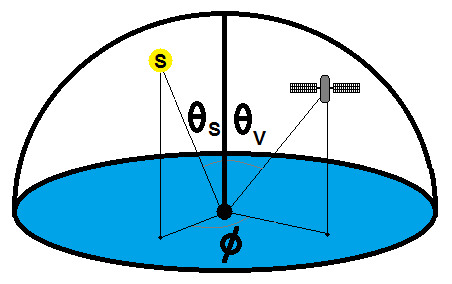
\includegraphics[width=0.5\textwidth]{int/figures/obs_ilum}
        \caption[Ángulos geométricos de observación-iluminación.]{Definición de los ángulos cenitales solar ($\theta_{s}$), de observación ($\theta_{v}$) y acimutal relativo sol-sensor ($\phi$), según la convención utilizada en esta tesis.}
        \label{int:obs_ilum}
        \end{figure}
    
        En general en teledetección se define la dirección en la cual se propaga la radiación en coordenadas esféricas, tomando como dirección polar el cenit; por lo que $\theta$ representa el ángulo cenital. El ángulo acimutal relativo $\phi$ se mide en sentido antihorario respecto del cenit desde el \textit{plano principal solar}, es decir, asumiendo un ángulo acimutal solar $\phi_{s}=0$. En el esquema de la Figura \ref{int:obs_ilum}, se determinan las dos direcciones más pertinentes: la del limbo solar y la de observación. En las definiciones dadas a continuación, donde aparezca la dupla $(\theta,\phi)$, esta referirá a una dirección de campo genérica, que podrá ser identificada con la dirección en que esté observando el sensor.

	\subsection{Irradiancia}
    \label{int:s:irradiancia}
        Considérese un flujo de energía radiativa atravesando un diferencial $dS$ de superficie plana. La tasa de flujo de energía radiativa, o potencia, por unidad de superficie se denomina \textit{irradiancia}, $E$, y es expresada en términos de energía neta $d^{2}U$ que atraviesa la superficie $dS$ en el intervalo temporal $[t,t+dt]$, o bien la potencia neta $d\Phi$ o \textit{flujo radiante} que atraviesa la superficie $dS$ como

        \begin{equation}
         E=\frac{d^{2} U}{dS\,dt}=\frac{d\Phi}{dS}\quad [W \cdot m^{-2}]
        \label{int:eq:irradiancia}
        \end{equation}

        La cantidad $d\Phi$ es diferencial de primer orden, considerada \textit{positiva} si el flujo radiante egresa del hemisferio superior (ascendente, $u$, suponiendo que la superficie sea horizontal) y \textit{negativa} en caso contrario (descendente, $d$). Es conveniente separar el flujo radiante en dos aportes positivos según si es ascendente o descendente, $d\Phi_{u}$ y $d\Phi_{d}$, cada uno de los cuales aporta una cantidad positiva de energía. Las irradiancias ascendente y descendente se definen entonces como
        
        \begin{equation}
         E_{u}=\frac{d\Phi_{u}}{dS}, \quad
         E_{d}=\frac{d\Phi_{d}}{dS}\quad [W\cdot m^{-2}]
        \label{int:eq:irrad_ascen_descen}
        \end{equation}
        
        El flujo radiante neto en la dirección ascendente es $d\Phi=d\Phi_{u}-d\Phi_{d}$. De la misma manera, la irradiancia neta es escrita como la diferencia entre dos cantidades positivas: $E=E_{u}-E_{d}$, siendo estas las medidas de toda la REM que sale y llega a una superficie, respectivamente (Figura \ref{int:irradiancia}).
        
        \begin{figure}
        \centering
        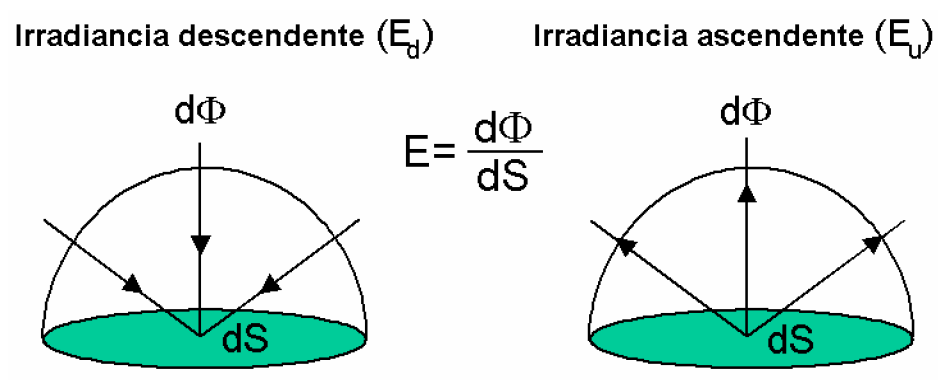
\includegraphics[width=0.6\textwidth]{int/figures/irradiancia}
        \caption[Esquematización de las irradiancias descendente ($E_{d}$) y ascendente ($E_{u}$).]{Esquematización de las irradiancias descendente ($E_{d}$) y ascendente ($E_{u}$), donde $d\Phi$ es el flujo radiante que llega a la superficie $dS$.} 
        \label{int:irradiancia}
        \end{figure}

	\subsection{Radiancia}
	\label{int:s:radiancia}
        Los sensores remotos tienen un campo limitado de observación y no detectan toda la irradiancia emitida por una superficie debido a que la forma del detector y su geometría de observación limitan la señal a una pequeña fracción del flujo. Esto implica que la dependencia del flujo radiante en función de la dirección tendrá un impacto sobre la energía detectada.
        %
        Teniendo en cuenta esto, consideremos un flujo radiante $d^{2}\Phi$ dentro de un ángulo sólido $d\Omega$ alrededor de la dirección $\hat{\Omega}$, atravesando un diferencial de superficie plana $dS$ (por ej. la superficie de un colector \textit{plano}) cuya orientación queda determinada por su normal $\hat{z}$ (ver Figura \ref{int:radiancia}). El ángulo comprendido entre $\hat{z}$ y la dirección de propagación $\hat{\Omega}$ es $\theta$. La potencia por unidad de superficie y por unidad de ángulo sólido se denomina \textit{radiancia}, $L(\theta,\phi)$, y viene dada por:
        
        \begin{equation}
         L(\theta,\phi)=\frac{d^{2}\Phi}{cos(\theta)dS\,d\Omega}\quad [W\cdot m^{-2} \cdot sr^{-1}]
        \label{int:eq:radiancia}
        \end{equation}

        \begin{figure}
        \centering
        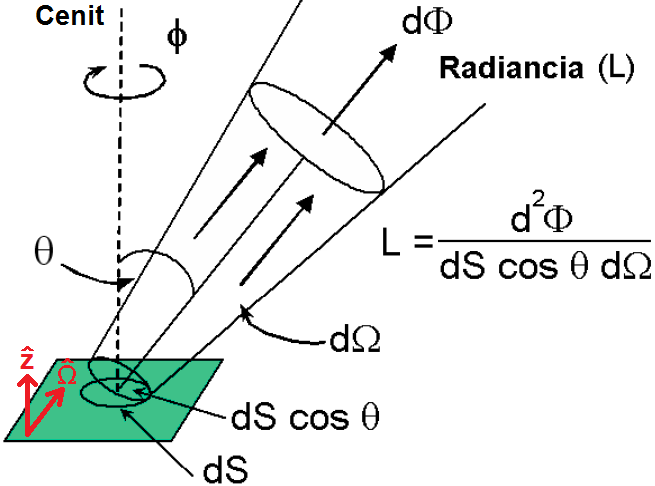
\includegraphics[width=0.6\textwidth]{int/figures/radiancia}
        \caption[Esquematización de la radiancia, $L(\theta,\phi)$, saliente de una superficie.]{Esquematización de la radiancia, $L(\theta,\phi)$, saliente de una superficie. Aquí, $dS$ representa el área de un elemento de la superficie, $L(\theta,\phi)$ es la radiancia que sale de $dS$ con un ángulo cenital $\theta$ (relativo a la normal $\hat{z}$) y un ángulo acimutal $\phi$. Su valor es definido por el flujo radiante que sale de $dS$ dentro del ángulo sólido $d\Omega$, centrado en la línea definida por $\theta$ y $\phi$.} 
        \label{int:radiancia}
        \end{figure}

        Nótese que, además de haber dividido por $d\Omega dS$, se ha dividido por el factor $cos(\theta) = \hat{z}\cdot \hat{\Omega}$, es decir, la proyección del elemento de superficie al plano normal a $\hat{\Omega}$. Es por esto que un colector de radiación plano se denomina \textit{colector coseno}. Nótese también que si $\hat{z}$ y $\hat{\Omega}$ apuntan en hemisferios opuestos, entonces $\hat{z}\cdot \hat{\Omega}$ es negativo. El flujo radiante es también negativo en este caso, por definición; por lo que la relación $d^{2}\Phi/cos(\theta)$ se mantiene positiva: la radiancia es siempre positiva.             Se obtendrá la relación entre radiancia e irradiancia a partir de la Ec. \ref{int:eq:radiancia}, que se podrá reescribir como

        \begin{equation}
         d^{2}\Phi=L(\theta,\phi)cos(\theta) dS d\Omega
        \label{int:eq:radiancia_dif}
         \end{equation}
        
        Utilizando las Ecs. \ref{int:eq:irradiancia} y \ref{int:eq:radiancia_dif} se obtienen las siguientes relaciones entre irradiancias (ascendente y descendente) y radiancia:

        \begin{equation}
        E_{u}=\left|\frac{d\Phi_{u}}{dS}\right|=\int_{+}d\Omega L(\theta,\phi)cos(\theta),\quad  E_{d}=\left|\frac{d\Phi_{d}}{dS}\right|= - \int_{-}d\Omega L(\theta,\phi)cos(\theta)
        \label{int:eq:rad_irrad1}
        \end{equation}
        
        \noindent donde + y - indican que se integra sobre los hemisferios superior e inferior, respectivamente. Sendas magnitudes son definidas positivas. Combinándolas, se obtiene que \textit{la irradiancia neta es la integración de la radiancia sobre todo el ángulo sólido},
        
        \begin{equation}
         E=E_{u} + E_{d}=\int_{4\pi}d\Omega L(\theta,\phi)|cos(\theta)|\quad [W\cdot m^{-2}]
        \label{int:eq:rad_irrad2}
         \end{equation}
        

        % \begin{enumerate}
        % \item \textbf{Radiancia proveniente del limbo solar}. En caso de despreciar el ángulo sólido abarcado por el limbo solar en el cielo terrestre, la radiancia solar incidente, previa a interactuar con la atmósfera, puede ser escrita como
        
        % \begin{equation}
        % L_{s}(\theta,\phi)(\hat{\Omega})=E_{s}\delta(\hat{\Omega}-\hat{\Omega}_{s})
        % \label{limbosolar}
        %  \end{equation}
        
        % \noindetsiendo siendo $\hat{\Omega}_{s}=(\theta_{s}, \phi_{s}=0)$ la dirección en la que se halla el limbo solar, $\delta(\hat{\Omega}-\hat{\Omega}_{s})=\delta(\phi)\delta(cos \theta - cos \theta_{s})$ la distribución delta de Dirac bidimensional, y $E_{s}$ la irradiancia solar extraatmosférica.
        
        A continuación, describiremos dos casos límite en la distribución angular de la radiancia: 

        \subsubsection{Radiancia saliente de una superficie lambertiana}
        \label{int:s:lambertiana}
        
            En caso de incidir sobre una superficie horizontal que sea un difusor perfecto, o sea una superficie que emite o refleja la energía con la misma intensidad en todas las direcciones independientemente del ángulo con el que incide la radiación, tendríamos, en las cercanías de la misma, siguiendo la Ec. \ref{int:eq:rad_irrad1},
            
            \begin{equation}
            E_{u}=E_{d}=\pi L
            \label{int:eq:lambertiana}
            \end{equation}
            
            A este tipo de superficies se las llama \textit{lambertianas} (Figura \ref{int:lambertiana}a).
            Ninguna superficie es perfectamente lambertiana, pero muchas de ellas, especialmente las opacas, se aproximan bastante (como la placa Spectralon utilizada en algunas mediciones radiómetricas de campo, ver \S \ref{dat:s:asdMed}).
        
        \subsubsection{Radiancia saliente de una superficie especular}
        \label{int:s:especular}
        
            Como caso opuesto a una superficie lambertiana puede mencionarse la superficie especular (Figura \ref{int:lambertiana}b). En este tipo de superficie la energía es reflejada con un ángulo igual al incidente pero en sentido opuesto, por lo que podremos afirmar que
            
            \begin{equation}
            L_{u}(\theta,\phi, z = 0^{+}) \propto L_{d}(\theta,-\phi, z = 0^{+})
            \label{int:eq:especular}
            \end{equation}
            
            \noindent donde hemos asumido una superficie planar horizontal. Una superficie natural que se aproxima bastante a este límite es la interfase agua-aire de una laguna profunda de aguas claras un día sin viento y vista en el rango NIR - donde valdría el supuesto de agua negra. En tal caso, la interfase se comportaría como un espejo que reflejaría siguiendo las leyes de Fresnel. Las superficies naturales en general se comportan de forma intermedia entre los casos lambertiano y especular (Figura \ref{int:lambertiana}c).
            
            \begin{figure}
            \centering
            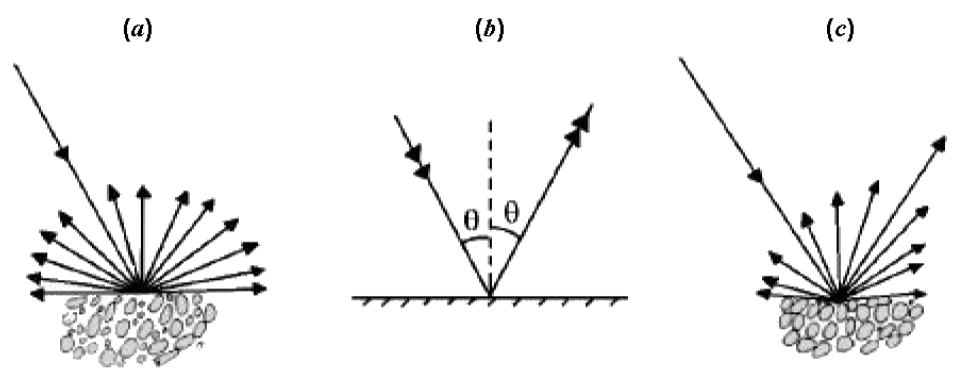
\includegraphics[width=0.75\textwidth]{int/figures/lambertiana}
            \caption[Diferentes tipos de superficies reflectoras: difusa, especular y mixta.]{Diferentes tipos de superficies reflectoras: (a) difusa o lambertiana, (b) especular y (c) tipo mixta.} 
            \label{int:lambertiana}
            \end{figure}
            % \end{enumerate}
        
	\subsection{Reflectancia y color del mar}
	\label{int:s:reflectancia}

        Todas las propiedades ópticas del agua varían con la longitud de onda ($\lambda$), por lo tanto se definen la irradiancia espectral, $E(\lambda)$, y la radiancia espectral, $L(\lambda,\theta,\phi)$, de manera análoga pero considerando radiación en el rango espectral diferencial $[\lambda,\lambda+d\lambda]$, es decir:

        \begin{align}
         &E(\lambda)=\frac{d E}{d\lambda}(\lambda) \quad [W m^{-2} nm^{-1}] \\
         &L(\lambda,\theta,\phi)=\frac{d L}{d\lambda}(\lambda,\theta,\phi) \quad [W m^{-2} sr^{-1} nm^{-1}]
        \label{int:eq:depEspectral}
        \end{align}
        
        La magnitud radiométrica de base del color del mar está determinada por la variación espectral de la reflectancia superficial irradiante o \textit{reflectancia del agua}, $\rho_{w}(\lambda)$, definida como el cociente entre la irradiancia ascendente, $E_{u}$, y la irradiancia descendente, $E_{d}$, justo por encima del agua ($z=0^{+}$), o sea:
        
        \begin{equation}
        \rho_{w}(\lambda)=\frac{E_{u}(\lambda,z=0^{+})}{E_{d}(\lambda,z=0^{+})} \quad [s/u]
        \label{int:eq:reflectancia}
        \end{equation}
        
        Dicha normalización por la irradiancia descendente le confiere a la reflectancia del agua la cualidad de propiedad óptica (cuasi) inherente (\textit{Inherent Optical Property}, IOP), es decir, (casi) independiente de las condiciones específicas del campo de iluminación (ángulo de incidencia del sol, estado de la atmósfera, etc.). Es por esto que la reflectancia es la magnitud radiométrica de la que se parte para la estimación de las diferentes sustancias presentes en el agua; aunque en realidad los sensores remotos no miden la irradiancia ascendente completa - presente en la Ec. \ref{int:eq:reflectancia} -; sino una porción de la misma. Por esto, muchas veces se prefiere expresar el color intrínseco del mar en función de la reflectancia sensada remótamente, $R_{rs}$:
        
        \begin{equation}
        R_{rs}(\theta,\phi,\lambda)=\frac{L_{u}(\theta,\phi,\lambda,z=0^{+})}{E_{d}(\lambda,z=0^{+})} \quad [sr^{-1}]
        \label{int:eq:rrs}
        \end{equation}
        
        \noindent pudiéndose establecer, en caso de asumir la superficie del agua como lambertiana (Ec. \ref{int:eq:lambertiana}), que

        \begin{equation}
        \rho_{w}(\lambda)=\pi R_{rs}(\lambda)
        \label{int:eq:rrsVsRho}
        \end{equation}

\section{El problema de la corrección atmosférica}
\label{int:s:componentes}
    
    Para poder esbozar más detalladamente cuál es el objetivo de aplicar una CA sobre imágenes de color es necesario conocer cuáles son las componentes que afectan la señal que arriba al sensor. La radiancia \textit{que arriba al sensor a TOA} (\textit{Top Of Atmosphere} en inglés) tras haber interactuado con el sistema óptico atmósfera-océano puede modelarse como la suma de diferentes términos que provienen de cada una de las diferentes componentes físicas del sistema. Una posible forma de descomponerla es:
    
    \begin{equation}
        L_{TOA} = L_{R} + [L_{A}+L_{RA}] + L_{g,TOA} + L_{sky,TOA} + L_{wc,TOA} + L_{w,TOA}
        \label{int:eq:ltoa}
    \end{equation}

    \noindent donde cada uno de los términos del lado derecho corresponden a radiancias conformadas por flujos de fotones que interactúan con las siguientes componentes:
    
    \begin{enumerate}
        \item $L_{R}$: fotones que fueron dispersados por moléculas de aire (y no arribaron a superficie).
        \item $L_{A}$: fotones que fueron dispersados por aerosoles (y no arribaron a superficie).
        \item $L_{RA}$: fotones que fueron dispersados por aerosoles y moléculas (dispersión indefectiblemente múltiple).
        \item $L_{g,TOA}$: fotones reflejados especularmente por la interfase del agua, provenientes directamente del limbo solar (\textit{sunglint}).
        \item $L_{sky,TOA}$: fotones reflejados especularmente por la interfase del agua, provenientes del campo de iluminación difusa del cielo (\textit{skyglint}).
        \item $L_{wc,TOA}$: fotones provenientes de la espuma que se halla en la superficie (\textit{whitecaps}).
        \item $L_{wc,TOA}$: fotones que fueron retrodispersados y reemergen del interior del cuerpo de agua.
    \end{enumerate}

    Es fundamental notar aquí que la radiancia es una Propiedad Óptica Aparente (\textit{Apparent Optical Property}, AOP), es decir, depende fuertemente del campo de iluminación. Para poder llegar a una expresión que contenga reflectancias (cuasi-IOPs), es necesario normalizar la expresión de la Ec. \ref{int:eq:ltoa} por la radiancia solar descendente a TOA, que no se mide si no que se calcula según:

    \begin{equation}
        E_{d,TOA} = F_{0}\left(\frac{R_{0}}{R}\right)^{2}cos(\theta_{s})
        \label{int:eq:edtoa}
    \end{equation}

    \noindent donde $F_{0}$ es la irradiancia solar extraatmosférica cuando el Sol se halla a $R_{0} = 1$ unidad astronómica de la Tierra (Figura \ref{int:hiper_thuillier}); el factor $\left(\frac{R_{0}}{R}\right)^{2}$ es el factor de adecuación de la irradiancia solar a la distancia real Sol-Tierra que varía con el día del año, siendo $R$ la distancia Tierra-Sol (Ley del Cuadrado Inverso de la Distancia) y $cos(\theta_{s})$ es el factor de corrección por el apartamiento del Sol del cenit (Ley del Coseno de Lambert). Considerando esta expresión para la irradiancia descendente a TOA, se define la reflectancia a TOA, $\rho_{TOA}$ siguiendo la Ec. \ref{int:eq:reflectancia} como

    \begin{equation}
        \rho_{TOA} = \frac{E_{u,TOA}}{E_{d,TOA}}\approx \frac{\pi L_{TOA}}{F_{0}\left(\frac{R}{R_{0}}\right)^{2}cos(\theta_{s})}
        \label{int:eq:rhotoa0}
    \end{equation}

    \begin{figure}
    \centering
    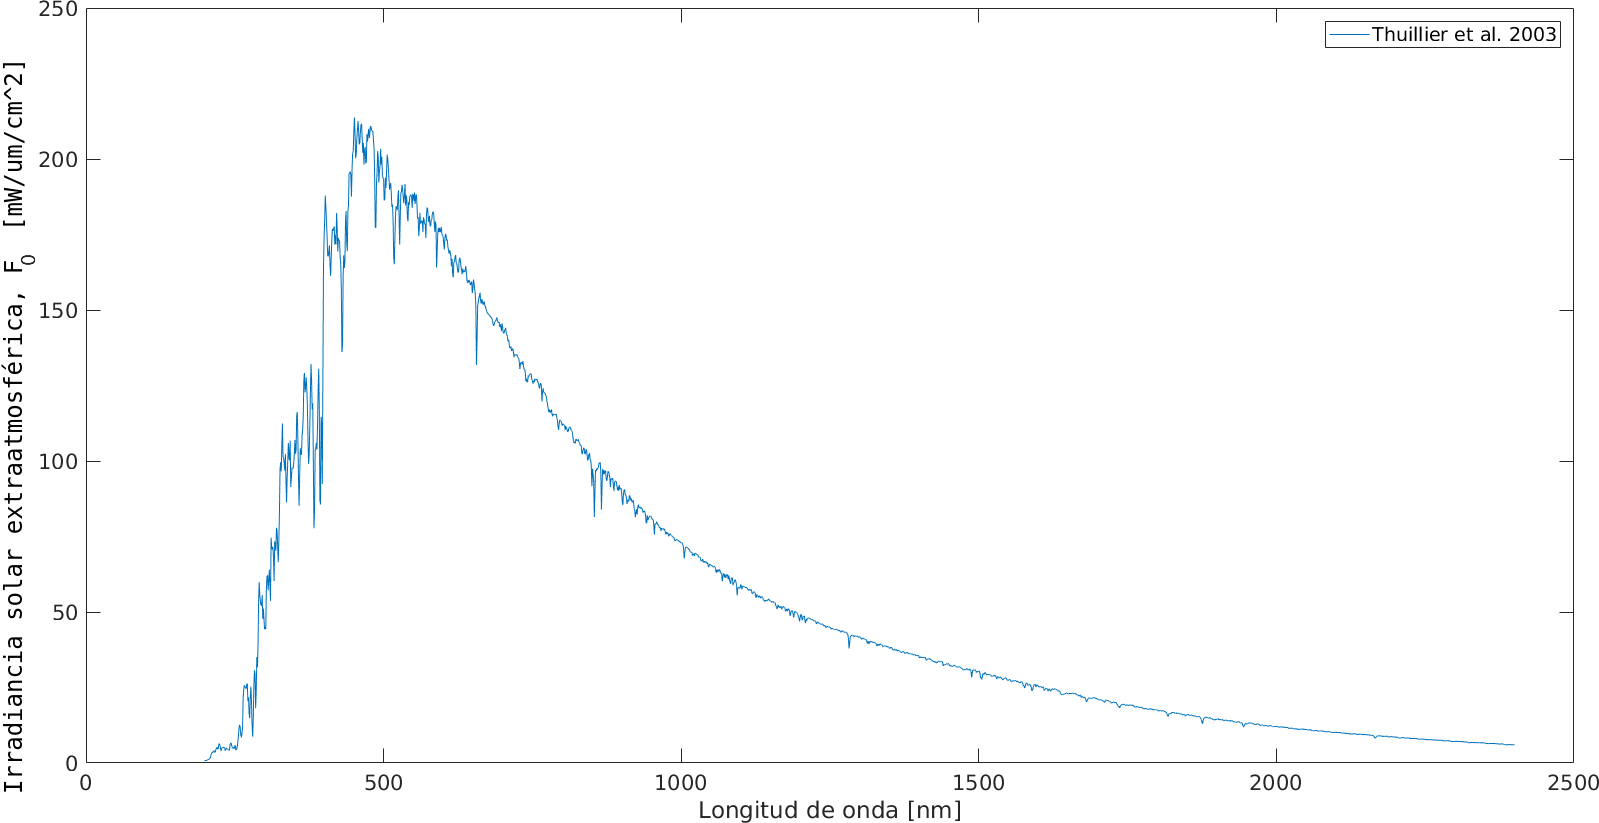
\includegraphics[width=\textwidth]{int/figures/hiper_thuillier.png}
    \caption[Irradiancia solar extraatmosférica (a $R = 1 UA$).]{Irradiancia solar extraatmosférica (a $R = 1 UA$) media medida por el espectrómetro SOLSPEC, Thuillier et al. 2003, \cite{thuillier2003}}
    \label{int:hiper_thuillier}
    \end{figure}

    \noindent donde el factor $\pi$ se utiliza como coeficiente de proporcionalidad entre la radiancia a TOA e irradiancia a TOA, es decir, se asume que la superfcie terrestre es  lambertiana (Ec. \ref{int:eq:lambertiana}). Si bien esta hipótesis no es válida, la expresión dada en Ec. \ref{int:eq:rhotoa0} se suele aplicar como convención y luego se aplica una corrección para minimizar el error introducido por esta hipótesis intentando reproducir la real Función de Distribución Bidireccional de la Reflectancia (\textit{Bidirectional Reflectance Distribution Function}, BRDF). Dicha corrección se suele aplicar directamente sobre la reflectancia del agua siguiendo el procedimiento culminado en Morel y Gentili 2002, \cite{morel2002}. Si embargo, en cuerpos de agua turbios como el RdP no se aplica debido a que dicha corrección fue diseñada para aguas ópticamente claras, y en caso de aplicarla introduciría mayor error en las estimaciones de reflectancias del agua (véase por ej. Li et al. 2019, \cite{li2019}). Una vez aplicado este factor, la expresión dada en la Ec. \ref{int:eq:ltoa} se puede expresar idénticamente, pero en reflectancias:

    \begin{equation}
        \rho_{TOA} = \rho_{R} + [\rho_{A} + \rho_{RA}] + \rho_{g,TOA} + \rho_{wc,TOA} + \rho_{w,TOA}
        \label{int:eq:rhotoa1}
    \end{equation}

    \noindent donde el término de \textit{skyglint} no figura pues fue incluido dentro del término $\rho_{R}$, dado que será corregido junto con la corrección por Rayleigh (véase \S \ref{int:s:rayleigh}). Es importante notar aquí que el sufijo \textit{TOA} que figura en los términos de superficie indica que dichas reflectancias no siguen exactamente la definición de reflectancia dada en la Ec. \ref{int:eq:reflectancia}, dado que no corresponden al cociente de irradiancias de salida y de entrada justo por encima de la superficie ($0^{+}$), sino al cociente a TOA. Para saber cómo relacionar estos términos con reflectancias de superficie reales es necesario establecer la relación entre las irradiancias a TOA y las irradiancias a $0^{+}$. Esto suele hacerse intoduciendo factores de \textit{transmitancia} que representan el efecto de la atmósfera sobre los términos de superficie. Por ejemplo, para el término de reflectancia del agua, se tiene que:

    \begin{equation}
        \rho_{w}(0^{+}) = \frac{E_{w}(0^{+})}{E_{d}(0^{+})} = \frac{\pi L_{w}(0^{+})}{E_{d,TOA}t_{s}t_{gs}} = \frac{\pi \frac{L_{w,TOA}}{t_{v}t_{gv}}}{E_{d,TOA}t_{s}t_{gs}} 
        \label{int:eq:rhowsupVStoa0}
    \end{equation}

    \noindent donde $E_{w}(0^{+})$ y $L_{w}(0^{+})$ son la radiancia y la irradiancia ascendente, medidas justo por encima de la superficie del agua; $t_{gs}$ y $t_{gv}$ son las transmitancias debidas a la absorción de moléculas de aire (véase \S \ref{int:s:tAbs}) en los caminos del Sol a la superficie y de la superficie al sensor, y $t_{s}$ y $t_{v}$ son las \textit{transmitancias difusas} (véase \S \ref{int:s:tDif}) - aplicables a radiancias lambertianas - debidas a fenómenos dispersivos en la atmófera. Obsérvese que nuevamente hemos asumido una relación entre la irradiancia y la radiancia asociada a la presencia de una superficie reflectora lambertiana. También es importante notar que las transmitancias son coeficientes que toman valores en el rango $[0-1]$, es decir que en general $t<1$ - pero cercana a 1 en ciertas regiones del espectro que se utilizan para el sensoramiento remoto usualmente llamadas \textit{ventanas atmosféricas} - por lo que, naturalmente $E_{d}(0+)<E_{d,TOA}$ y $L_{w}(0+)>L_{w,TOA}$. Es evidente que, reordenando la Ec. \ref{int:eq:rhowsupVStoa0}, obtenemos la siguiente relación:

    \begin{equation}
        \rho_{w}(0^{+}) = \frac{\rho_{w,TOA}}{t_{s}t_{v}t_{gs}t_{gv}}
        \label{int:eq:rhowsupVStoa}
    \end{equation}

    Debido a que el término de espuma (\textit{WC}) es aproximadamente lambertiano, \cite{gordon1994b}, la relación entre $\rho_{wc}(0^{+})$ y $\rho_{wc,TOA}$ es equivalente a la dada en Ec. \ref{int:eq:rhowsupVStoa0}. Por otro lado, el término debido al \textit{sunglint} corresponde al caso de una reflexión especular (Ec. \ref{int:eq:especular}), por lo que el factor que se aplica para representar el acople del \textit{sunglint} con la dispersión atmosférica es el de \textit{transmitancia directa}, $T$ (véase \S \ref{int:s:tDir}), resultando entonces

    \begin{equation}
        \rho_{g}(0^{+}) = \frac{\rho_{g,TOA}}{T_{ds}T_{dv}t_{gs}t_{gv}}
        \label{int:eq:rhogsupVStoa}
    \end{equation}
    
    La absorción de moléculas de aire también afectará a los términos atmosféricos puros y podremos desacoplarla - en los casos del ozono ($O_{3}$) y el dióxido de nitrógeno ($NO_{2}$) estratosféricos - de los efectos dispersivos (mayormente troposféricos, \S \ref{int:s:tAbs}), de forma tal que

    \begin{equation}
        \rho_{R} + [\rho_{A} + \rho_{RA}] = (\rho_{r} + [\rho_{a} + \rho_{ra}])t_{gs}t_{gv}
        \label{int:eq:rhorAbs}
    \end{equation}

    \noindent donde las reflectancias con subíndices minúsculos representan a los fenómenos dispersivos en ausencia de absorción de moléculas de aire. Tras haber considerado todos estos procesos, la descomposición de la reflectancia a TOA puede escribirse como

    \begin{equation}
        \rho_{TOA} = \underbrace{t_{g}}_\text{A}.(\underbrace{\rho_{r}}_\text{B} + \underbrace{[\rho_{a} + \rho_{ra}]}_\text{C} + \underbrace{T}_\text{D}.\underbrace{\rho_{g}}_\text{E} + \underbrace{t}_\text{F}.[\underbrace{\rho_{wc}}_\text{G} + \underbrace{\rho_{w}}_\text{H}])
        \label{int:eq:rhotoa}
    \end{equation}

    \noindent donde hemos expresado las transmitancias sol-superficie (\textit{s}) y superficie-sensor (\textit{v}) en transmitancias de dos caminos, por ej. $t = t_{s}t_{v}$. El objetivo de la corrección atmosférica radica en aislar el término $\rho_{w}$ (H) del resto de los términos, originados en la atmósfera y en la interfase aire-agua (A-G). A continuación, para cada uno de estos términos, haremos una breve caracterización de sus propiedades, así como de los esquemas estándares de estimación para su corrección aplicados a cada uno. Es importante destacar que en este análisis obviaremos otros pasos estándares de CA, todos detallados en el tutorial de Mobley et al. 2016, \cite{mobley2016}, y descritos muy brevemente a continuación:
    
    \begin{enumerate}
        \item \textbf{Calibración vicaria}. Típicamente, las reflectancias del agua obtenidas tras aplicar una CA sobre una imagen de color no son exactamente coincidentes con las reflectancias medidas por radiómetros de campo debido a inexactitudes en el proceso de corrección, degradación de diferentes componentes del sensor satelital o inexactitudes en las mediciones \textit{in situ}. Es por esto que típicamente se utilizan sitios de calibración específicos que cuentan con mediciones de campo - tanto de la reflectancia del agua como del estado de la atmósfera - que se asumen como verdaderas (\textit{ground-truth}) y, estableciendo el apartamiento entre las mediciones de campo y las estimaciones satelitales, se computan coeficientes globales que se aplican directamente a las reflectancias del agua estimadas por el satélite. Esto se hace con el objetivo de que las estimaciones satelitales resulten lo más coincidentes posible con las mediciones de campo. Esto define una Calibración Vicaria del Sistema (\textit{System Vicarious Calibration}, SVC) - llamados así porque son calculados con el sensor en órbita - y son un proceso usual aplicado sobre las reflectancias del agua satelitales. Genéricamente corresponderá un conjunto diferente de coeficientes de calibración vicaria para cada esquema diferente de CA aplicada y para cada sensor.
        \item \textbf{Corrección por sensibilidad fuera de banda (\textit{Out-Of-Band sensitivity}, OOB)}. Las Funciones de Respuesta Espectral, (\textit{Spectral Response Function}, SRF), muchas veces toman valores no nulos en longitudes de onda muy alejadas a la central. En tal caso se computan factores de corrección que relacionan las SRFs reales - es decir, con sensibilidad OOB - con SRFs razonables que no consideren longitudes de onda demasiado alejadas de la nominal. Se discute en \cite{mobley2016} cuándo es importante aplicar dicha corrección y cuándo no.
        \item \textbf{Corrección por sensibilidad a la polarización}. Se debe aplicar debido a diferencias - indeseadas - en las mediciones de ciertos radiómetros de color debidas a diferentes estados de polarización de la radiación incidente. Típicamente se computa un factor de corrección, \cite{mobley2016}, basado en i) una caracterización pre-lanzamiento de la matriz de Mueller del sensor - que describe la sensibilidad a las diferentes polarizaciones -, y ii) en simulaciones de transferencia radiativa que consideran únicamente las componentes de más impacto en el grado de polarización dentro del balance de la Ec. \ref{int:eq:rhotoa}: la dispersión Rayleigh molecular y el \textit{sunglint}.
    \end{enumerate}

\section{Absorción molecular (A)}
\label{int:s:tAbs}

    Algunas de las componentes naturales del aire son absorbentes. Existen dos tipos de componentes absorbentes: las mayormente troposféricas (vapor de agua, $H_{2}O$, y oxígeno, $O_{2}$) y las mayormente estratosféricas (ozono, $O_{3}$ y dióxido de nitrógeno, $NO_{2}$).
    
    Dado que los fenómenos de dispersión atmosférica ocurren mayormente en la troposfera, la absorción debida a los gases troposféricos (oxígeno y vapor de agua) es más complicada de corregir, puesto que está fuertemente acoplada a los procesos de dispersión. Esto implica que, dado un fotón en la troposfera, el camino óptico recorrido en la atmósfera es difícil de computar dado que pudo estar sometido a múltiples procesos de dispersión; por lo que es difícil encontrar una expresión para el factor de transmitancia. Afortunadamente, las líneas de absorción de dichas moléculas en el visible son bastante angostas y pueden ser evitadas definiendo bandas que no se vean afectadas por las mismas (Figura \ref{int:oxigeno_h20_Mobley}).

    \begin{figure}
    \centering
    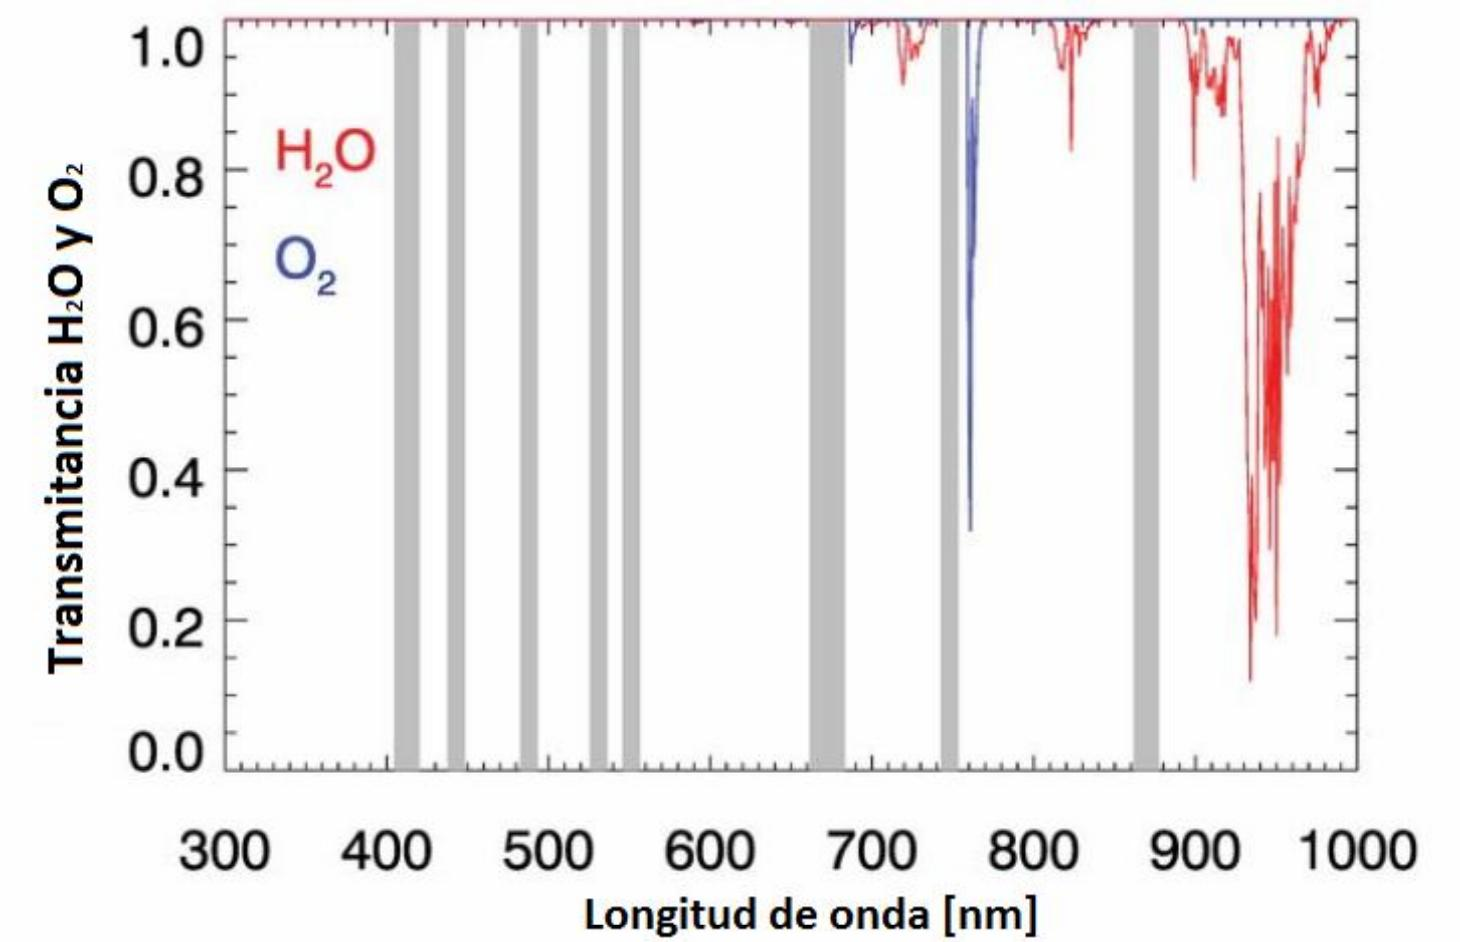
\includegraphics[width=0.7\textwidth]{int/figures/oxigeno_h20_Mobley.png}
    \caption[Transmitancias debidas a la absorción del oxígeno y del vapor de agua.]{Transmitancias debidas a la absorción del oxígeno, $O_{2}$, y del vapor de agua, $H_{2}O$ para una atmósfera húmeda tropical. La resolución es de 1 nm. Figura de Mobley et al. 2016, \cite{mobley2016}.}
    \label{int:oxigeno_h20_Mobley}
    \end{figure}

    Por el contrario, tanto el ozono como el dióxido de nitrógeno se hallan principalmente en la estratósfera, por lo que su acople con los procesos de dispersión es bajo y se podrá asumir la siguiente expresión:

    \begin{equation}
        t_{g}^{O_{3} + NO_{2}} = t_{g}^{O_{3}}(\lambda,[O_{3}],\mu) \times t_{g}^{NO_{2}}(\lambda,[NO_{2}],\mu)
        \label{int:eq:tAbsO3NO2}
    \end{equation}

    \noindent es decir, que el factor de transmitancia total dado por el efecto conjunto de $O_{3}$ y $NO_{2}$ podrá ser factoreado y estimado a partir de sus concentraciones, $[O_{3}]$ y $[NO_{2}]$, y el factor geométrico de masa de aire ($\mu$) dado por los ángulos cenitales de iluminación ($\theta_{s}$) y observación ($\theta_{v}$):
    
    \begin{equation}
        \mu = \frac{1}{cos(\theta_{s})} + \frac{1}{cos(\theta_{v})}
        \label{int:eq:mu}
    \end{equation}

    \noindent sin contemplar ningún efecto de acople con otros efectos atmosféricos, como la dispersión molecular o la presencia de aerosoles. A su vez, cada uno de estos factores puede expresarse a partir de sus respectivos coeficientes de extinción ($k$) según:

    \begin{equation}
        t_{g}^{O_{3} }(\lambda,[O_{3}],\mu) = e^{-k_{O_{3} }(\lambda)[O_{3} ]\mu}
        \label{int:eq:tAbsExpKCTCMU_O3}
    \end{equation}

    \begin{equation}
        t_{g}^{NO_{2}}(\lambda,[O_{3}],\mu) = e^{-k_{NO_{2}}(\lambda)[NO_{2}]\mu}
        \label{int:eq:tAbsExpKCTCMU_NO2}
    \end{equation}
    
    Los valores de $k_{O_{3}}$, expresado como el coeficiente de atenuación (en cm$^{-1}$) cada 1 nm entre 200 y 2550 nm, así como el $k_{NO_{2}}$, expresado como la sección eficaz de absorción del $NO_{2}$ (en cm$^{2}$/molécula) cada 1 nm entre 200 y 2540 nm, pueden ser obtenidos del sitio del \textit{Ocean Biology Processing Group} de la NASA \cite{obpg}. Es importante notar que las expresiones dadas en las Ecs. \ref{int:eq:tAbsExpKCTCMU_O3} y \ref{int:eq:tAbsExpKCTCMU_NO2} corresponden a transmitancias de dos sentidos (sol-superficie y superficie-sensor, tal como las que figuran en la Ec. \ref{int:eq:rhotoa}).
    
    Para computar los valores de los factores dados en la Ec. \ref{int:eq:tAbsO3NO2} es necesario conocer las concentraciones de ozono y dióxido de nitrógeno. Si bien estas pueden obtenerse a partir de datos de satelites meteorológicos (como el TOMS/EPTOMS - Total Ozone Mapping Spectrometer onboard the Earth Probe spacecraft - de la NASA), o de re-análisis (por ej. el provisto por el European Centre for Medium-Range Weather Forecasts, ECMWF), muchas veces no se dispone de dicha información, por lo que se deben asumir valores nominales de $[O_{3}]$ y $[NO_{2}]$. Los valores típicos son de:

    \begin{equation}
        [O_{3}] = 80.7\times10^{16} part/cm^{2} = 300 DU
        \label{int:eq:conc_o3}
    \end{equation}
    \begin{equation}
        [NO_{2}] = 1.1 \times10^{16} part/cm^{2}
        \label{int:eq:conc_no2}
    \end{equation}

    En la Figura \ref{int:O3_RDP_ECMWF} se puede observar la concentración de ozono provista por el re-análisis de ECMWF (cuyos mapas vienen distribuidos junto con las imágenes OLCI Nivel L1B de la ESA) que muestra una distribución espacialmente variable y con valores muy cercanos al valor nominal de 300 DU (Dobson Units). En la Figura \ref{int:O3_ECMWF_VS_NOM} se puede observar la transmitancia por absorción de ozono en 620 nm (la banda del sensor OLCI más afectada por dicho gas) calculada a partir del dato de concentración de ozono que viene con la imagen (izquierda) y a partir de una concentración nominal de 300 DU (derecha). Esta figura muestra que la variabilidad espacial del ozono tiene un pequeño impacto sobre la transmitancia en comparación con la variabilidad en el factor geométrico de masa de aire ($\mu$), que es determinado por la geometría de observación e iluminación.

    \begin{figure}
    \centering
    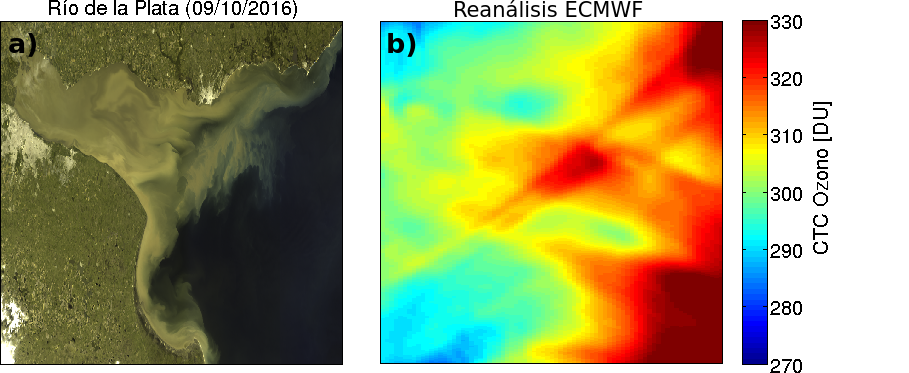
\includegraphics[width=\textwidth]{int/figures/O3_RDP_ECMWF.png}
    \caption[Concentración de ozono en DU obtenida del re-análisis de ECMWF para el RdP el día 09-OCT-2016.]{a) Composición RGB de OLCI (Sentinel-3A) del Río de la Plata del día 9 de octubre de 2016 (en geometría del sensor). b) Concentración de ozono en DU obtenida del re-análisis de ECMWF que es distribuido por la ESA dentro de los productos L1B.}
    \label{int:O3_RDP_ECMWF}
    \end{figure}

    \begin{figure}
    \centering
    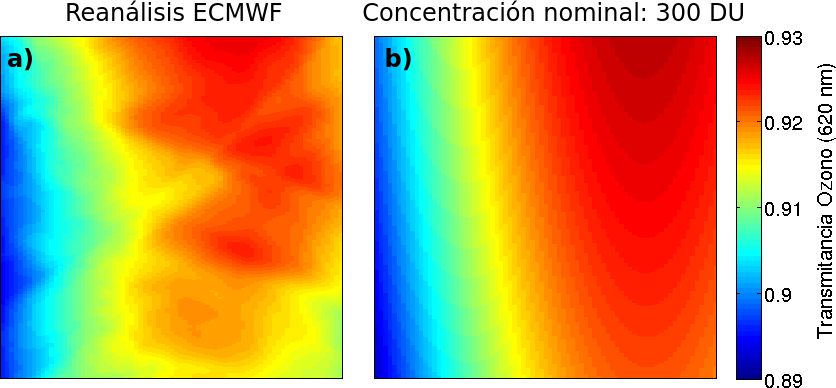
\includegraphics[width=\textwidth]{int/figures/O3_ECMWF_VS_NOM.png}
    \caption[Transmitacias debidas a la absorción del ozono a partir de concentración otorgada por ECMWF y de 300 DU (nominal).]{Transmitacias debidas a la absorción del ozono calculadas utilizando concentraciones provistas por el re-análisis de ECMWF (a) y una concentración nominal de ozono de 300 DU (b).}
    \label{int:O3_ECMWF_VS_NOM}
    \end{figure}

    Por otro lado, la Figura \ref{int:NO2} muestra el factor de transmitancia del $NO_{2}$ para las bandas del SABIA-Mar según diferentes concentraciones (CTC) y factores de masa ($\mu$). Obsérvese que, obviando las curvas asociadas al valor extremo de $[NO_{2}] = 6\times10^{16} part/cm^{2}$ (triángulos) que se corresponden a escenarios industriales donde existen niveles altos de $NO_{2}$ troposféricos, los escenarios naturales presentan valores superiores al $97\%$; por lo que es de esperar un error pequeño al asumir un valor nominal de $[NO_{2}] = 1.1\times10^{16} part/cm^{2}$ (asteriscos). Aparte, la expresión de la Ec. \ref{int:eq:tAbsExpKCTCMU_NO2} dejaría de ser válida en los escenarios con valores extremos de escenarios industriales debido a que la mayoría del $[NO_{2}]$ en estos casos se hallaría en las capas más bajas de la atmósfera.

    \begin{figure}
    \centering
    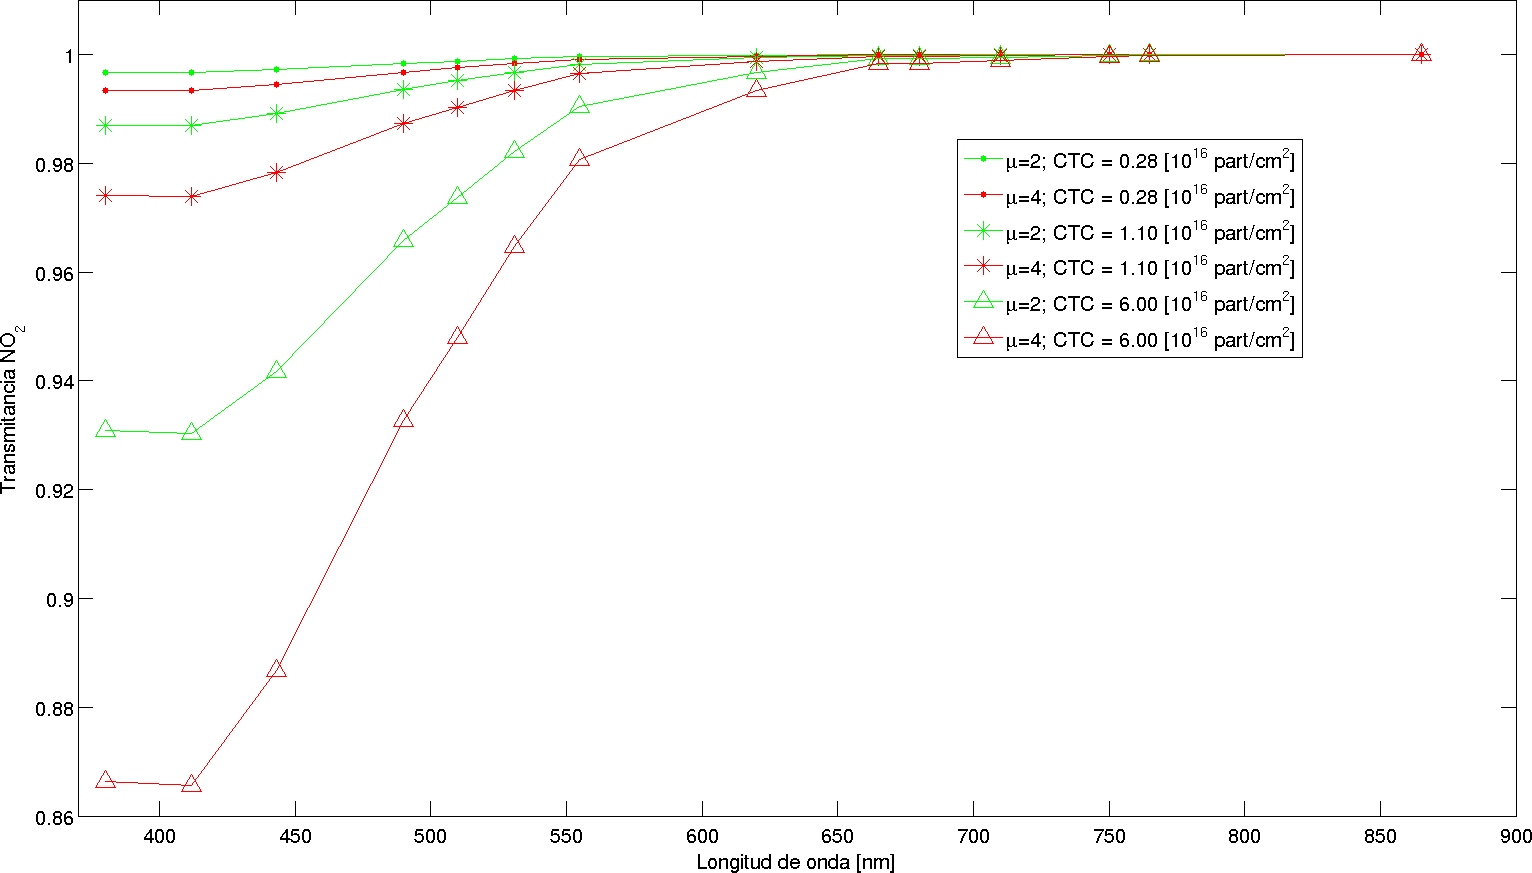
\includegraphics[width=\textwidth]{int/figures/NO2.png}
    \caption[Factor de transmitancia de NO$_{2}$ para diferentes concentraciones y factores de masa de aire.]{Factor de transmitancia de NO$_{2}$ para diferentes concentraciones y factores de masa de aire ($\mu$) para las bandas del SABIA-Mar.}
    \label{int:NO2}
    \end{figure}
    
    Cuando no se disponen de valores de concentración de gases absorbentes en la atmósfera, se pueden asumir los valores nominales de concentración de $O_{3}$ y $NO_{2}$ dados en las Ecs. \ref{int:eq:conc_o3} y \ref{int:eq:conc_no2}, como en Vanhellemont et al. 2014 \cite{vanhellemont2014}. De esta forma, y habiendo evadido las líneas de absorción de los gases troposféricos, se puede calcular un factor de transmitancia total gaseosa $t_{g}$ que sólo variará de acuerdo a la banda y al factor de masa ($\mu$):


    \begin{equation}
        t_{g}(\lambda) = t_{g}^{O_{3} + NO_{2}}(\lambda,\mu)
        \label{int:eq:tAbsO3NO2Nominal}
    \end{equation}

    En la Figura \ref{int:AbsorcionGaseosaHyper375_1700} se muestra la variabilidad hiper-espectral de la transmitancia gaseosa total en el rango $[375-1700]$ nm, y los valores ya integrados en las bandas del SABIA-Mar (Figura \ref{int:AbsorcionGaseosaSabiaMar}). En ambos casos, se hallan los valores obtenidos para factores de masa $\mu=2$ (observación e iluminación en cenit) y $\mu=4$ (observación e iluminación a $60\degree$ del cenit). 

    \begin{figure}
    \centering
    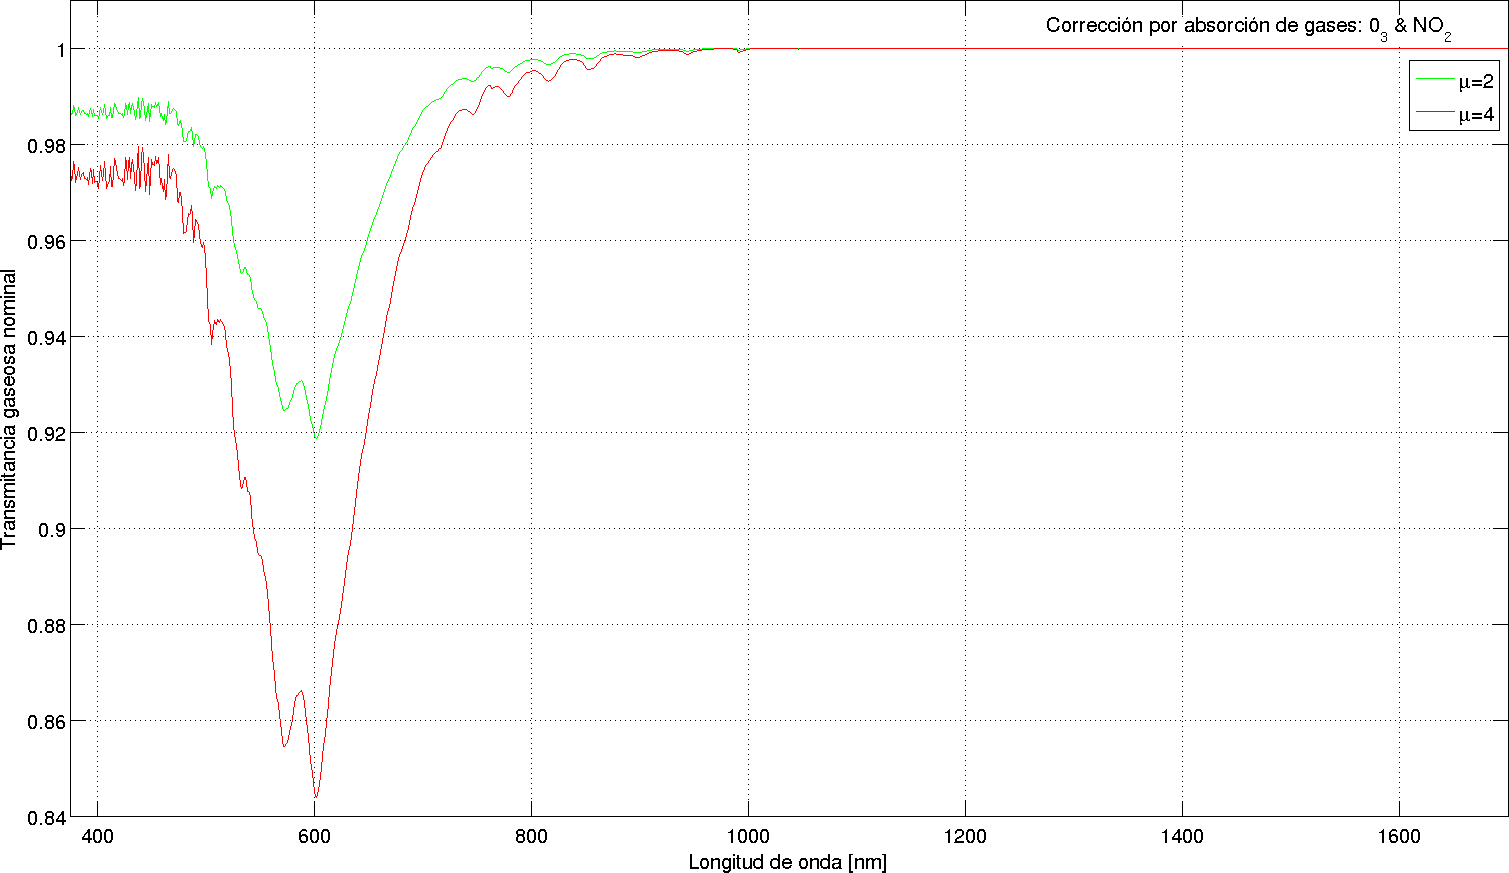
\includegraphics[width=\textwidth]{int/figures/AbsorcionGaseosaHyper375_1700.png}
    \caption[Transmitancia gaseosa por presencia de concentraciones nominales de ozono y dióxido de nitrógeno.]{Transmitancia gaseosa por presencia de concentraciones nominales de $O_{3}$ y $NO_{2}$ en el rango $[375-1700]$ nm: Valores obtenidos para factores de masa de aire $\mu = 2$ y $\mu = 4$.}
    \label{int:AbsorcionGaseosaHyper375_1700}
    \end{figure}

    \begin{figure}
    \centering
    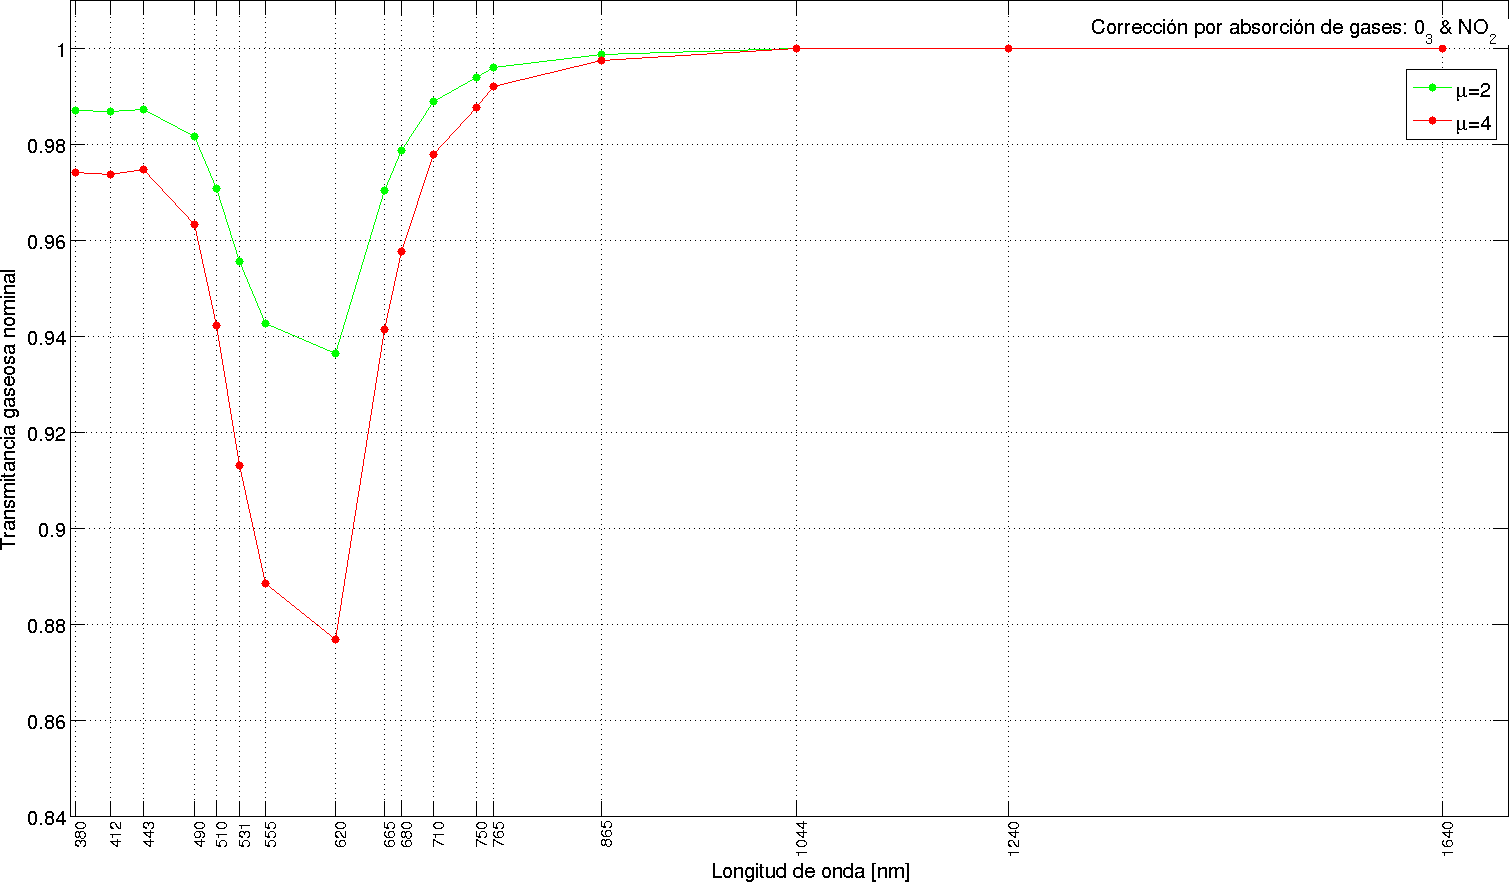
\includegraphics[width=\textwidth]{int/figures/AbsorcionGaseosaSabiaMar.png}
    \caption{Íd. Figura \ref{int:AbsorcionGaseosaHyper375_1700}, pero integrado sobre las SRFs de las bandas del SABIA-Mar.}
    \label{int:AbsorcionGaseosaSabiaMar}
    \end{figure}
    
\section{Dispersión Rayleigh molecular (B)}
\label{int:s:rayleigh}

    La dispersión de Rayleigh es la dispersión elástica de la luz visible o cualquier otra radiación electromagnética por partículas cuyo tamaño es mucho menor que la longitud de onda de los fotones dispersados. En la Teoría Clásica Electromagnética la dispersión de Rayleigh se genera como resultado de la polarizabilidad de las moléculas que actúan como centro dispersor. A partir de un campo de REM inducido por el efecto del campo REM incidente sobre las cargas de la partícula, las mismas actuarán como un dipolo eléctrico que oscilará a la misma frecuencia que la del campo incidente. La radiancia $L_{r} $ de la luz dispersada por una molécula de aire en un haz de luz de longitud de onda $\lambda$ y radiancia incidente $L_{0}$ viene dada por:

    \begin{equation}
        L_{r} = L_{0}{\frac {(1+cos^{2}(\Theta))}{2R^{2}}}\left({\frac{2\pi}{\lambda}}\right)^{4}\left({\frac{n^{2}-1}{n^{2}+2}}\right)^{2}\left({\frac{d}{2}}\right)^{6}
        \label{int:eq:Lray}
    \end{equation}

    \noindent donde $R$ es la distancia a la partícula, $\Theta$ es el ángulo de dispersión, $n$ y $d$ son el índice de refracción y el diámetro de la partícula, respectivamente. A partir del término $1+cos^{2}(\Theta)$, notamos que la dispersión de Rayleigh es simétrica y cuasi-isótropa (Figura \ref{int:scatteringTypes}). A su vez, notamos que la dispersión de Rayleigh es fuertemente dependiente de la longitud de onda ($\lambda^{-4}$).
    
    
    Si bien en ciertas circunstancias la radiancia de Rayleigh puede comprender entre el 50\% y el 90 \% de la radiancia total a TOA (Figuras \ref{int:RDP_TC_comparison_B_RHOGRC} y \ref{int:RDP_TC_comparison_B_RHO}), las propiedades ópticas de la dispersión de Rayleigh en la atmósfera son fácilmente calculables (con un error de $\sim 0.2\%$). En el contexto de la CA de imágenes de color del mar, para llevar a cabo la corrección por dispersión Rayleigh (\textit{Rayleigh Correction}, RC) se suelen utilizar simulaciones de Transferencia Radiativa (TR) para resolver la Ecuación Vectorial (polarizada) de Transferencia Radiativa (EVTR, \S \ref{sos:s:EVTR}) bajo la única presencia de moléculas dispersivas de aire y una superficie reflectora (que dará lugar al término de \textit{skyglint}). Dicho código de transferencia radiativa deberá incluir fenómenos de dispersión múltiple, polarización y un modelo de rugosidad de la interfase agua-aire. Típicamente, ésta se parametriza en función de la intensidad del viento, siguiendo la distribución de inclinaciones de facetas de la superficie propuesta por Cox y Munk 1954 \cite{coxmunk1954} (Figura \ref{int:coxmunk}):
    
    \begin{equation}
        g_{glitter}(\theta_{n},w) = \frac{1}{4\pi\sigma^{2}(w)cos^{2}(\theta_{n})}e^{-\left(\frac{tan(\theta_{n})}{\sigma(w)}\right)^{2}}
        \label{int:eq:coxmunk}
    \end{equation}
    
    \noindent siendo $\theta_{n}$ la orientación cenital de cada diferencial de superficie de agua - es decir, cada faceta -, $w$ la intensidad del viento en $m/s$ y $\sigma(w[m/s]) = 0.00300 + 0.00512w$.


    \begin{figure}
    \centering
    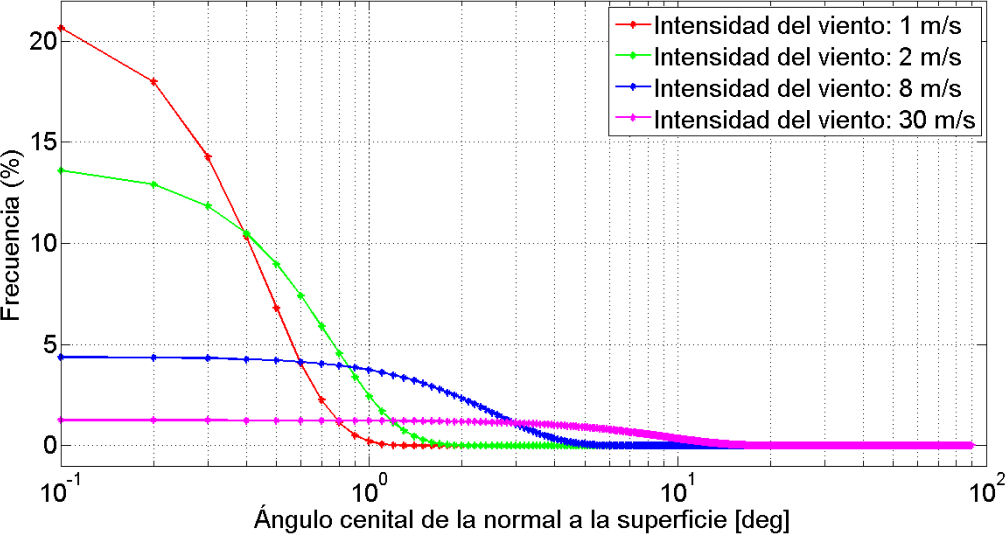
\includegraphics[width=\textwidth]{int/figures/coxmunk.png}
    \caption[Distribuciones de ángulos cenitales de las facetas de la interfase aire-agua para diferentes intensidades del viento en superficie.]{Distribuciones de ángulos cenitales formados por las direcciones normales de las facetas de la interfase aire-agua para diferentes intensidades del viento en superficie (Parametrización de Cox y Munk, \cite{coxmunk1954}). Un ángulo de $0\degree$ corresponde a una superficie horizontal. Paso de la distribución: $0.1\degree$.}
    \label{int:coxmunk}
    \end{figure}

    A su vez, para que el esquema de corrección por Rayleigh sea posible es necesario introducir los siguientes parámetros ópticos al código de transferencia radiativa:
    
    \begin{enumerate}
    
        \item \textbf{Cociente de depolarización molecular}, $\delta_{r}$. El mismo es una corrección debida a la anisotropía de las moléculas de aire. Este influye en las expresiones teóricas tanto de la matriz de fase (véase \S \ref{sos:s:matrizdefase}), inscripta dentro de la rutina de transferencia radiativa, como del espesor óptico. En general se utiliza la expresión dada por Bodhaine et al. 1999, \cite{bodhaine1999} (Figura \ref{int:rayleigh_tau_depol})
        
        \item \textbf{Espesor óptico molecular en superficie (Rayleigh)}, $\tau_{r}(\lambda, z = 0)$. El espesor óptico es el parámetro que indica la extinción de un haz de luz en una unidad de longitud dada (Ec. \ref{sos:eq:tau_definicion}). Existe una expresión teórica para el espesor óptico de Rayleigh, dada por \cite{bodhaine1999}:

        \begin{equation}
            \tau_{r}(\lambda, z = 0) = \frac{24 P N_{A}\pi^{3}(n^{2}-1)^{2}}{mg\lambda^{4}N^{2}(n^{2}-1)^{2}}\left(\frac{6+3\delta_{r}}{6-7\delta_{r}}\right)^{2}
            \label{int:eq:taur}
        \end{equation}

        \noindent siendo $n$ el índice de refracción del aire, $N$ la densidad molecular, $P$ la presión atmosférica en superficie y $N_{A}$ el número de Avogadro. El factor de la derecha (\textit{factor de King}) introduce la dependencia con $\delta_{r}$. Si bien esta expresión teórica es suficientemente adecuada para la corrección de Rayleigh aplicada a las imágenes de color, se utiliza típicamente el espectro reportado en Bodhaine et al. 1999, \cite{bodhaine1999} (Figura \ref{int:rayleigh_tau_depol}), al igual que el cociente de depolarización reportado por los mismos autores.

        \item \textbf{Altura característica de decaimiento exponencial}, $H_{r}$. En el cómputo de la reflectancia por dispersión Rayleigh, es necesario introducir la variación del espesor óptico molecular con la altura. Asumiendo una atmósfera isoterma y en balance hidrostático, el espesor óptico sigue un régimen exponencial decreciente con la altura:
    
        \begin{equation}
            \tau_{r}(\lambda, z) = \tau_{r}(\lambda, z = 0)e^{-z/H_{r}}
            \label{int:eq:hray}
        \end{equation}

        \noindent donde $z$ es la altura (en km) y típicamente, $H_{r} = 8$ km, siguiendo la ley barotrópica.
    \end{enumerate} 


    \begin{figure}
    \centering
    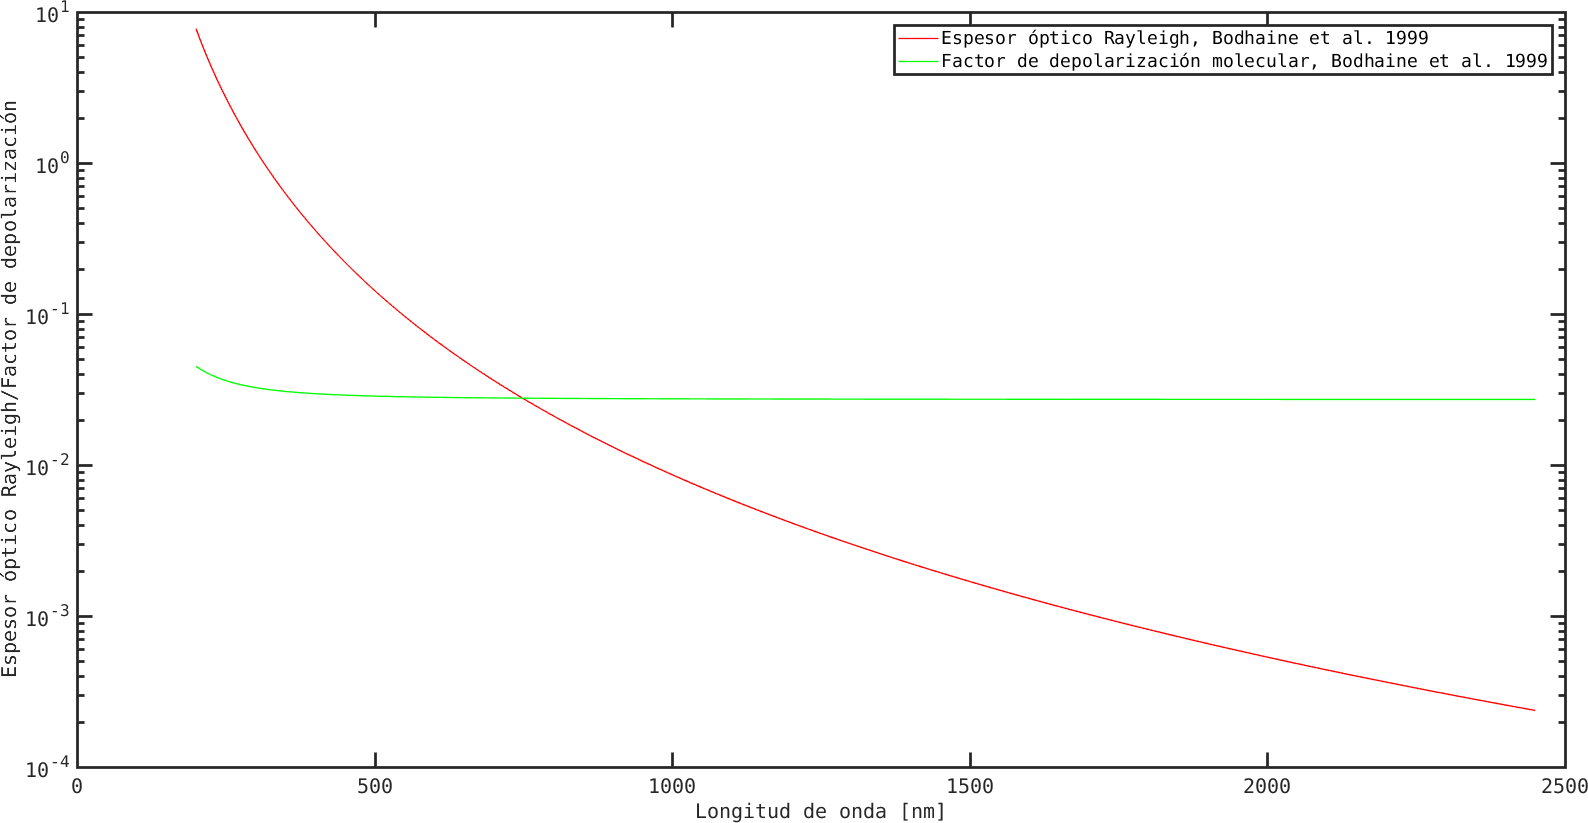
\includegraphics[width=\textwidth]{int/figures/rayleigh_tau_depol.png}
    \caption[Espesor óptico de Rayleigh y cociente de depolarización molecular.]{Espesor óptico de Rayleigh y cociente de depolarización molecular basados en Bodhaine et al. 1999, \cite{bodhaine1999}. [Graficado a partir del archivo bodhaine.txt que se halla en la página del OBPG de la NASA, \cite{obpg}].}
    \label{int:rayleigh_tau_depol}
    \end{figure}

    \begin{figure}
    \centering
    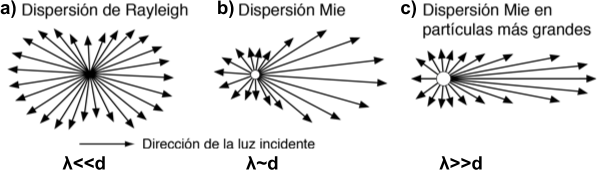
\includegraphics[width=0.75\textwidth]{int/figures/scatteringTypes.png}
    \caption[Distribución angular de la dispersión según la relación entre la longitud de onda y el tamaño de partícula.]{Distribución angular de la dispersión según la relación entre la longitud de onda ($\lambda$) y el tamaño de partícula ($d$): a) Dispersión tipo Rayleigh ($\lambda<<d$), b) tipo Mie ($\lambda \sim d$) y c) tipo Mie ($\lambda>>d$).}
    \label{int:scatteringTypes}
    \end{figure}

    En resumen, las reflectancias utilizadas para la corrección por Rayleigh (RC) se suelen obtener de tablas pre computadas (\textit{Look Up Tables}, LUTs) que dependen de los siguientes parámetros auxiliares:
    
    \begin{enumerate}
        \item Geometría de iluminación-observación (generalmente disponible con los productos satelitales).
        \item Velocidad del viento en superficie (necesaria para computar la rugosidad de la superficie, Ec. \ref{int:eq:coxmunk}).
        \item Presión atmosférica en superficie (necesaria para ajustar los valores de espesor óptico de Rayleigh, Ec. \ref{int:eq:taur})
    \end{enumerate}
    
    El detalle de cómo se efectúan estos cálculos en el procesador del OBPG de la NASA, SeaDAS (\textit{SeaWIFS Data Analysis System}) - utilizado en la presente tesis - se hallan descritos en Ahmad y Fraser 1982, \cite{ahmad1982}.

    \begin{figure}
    \centering
    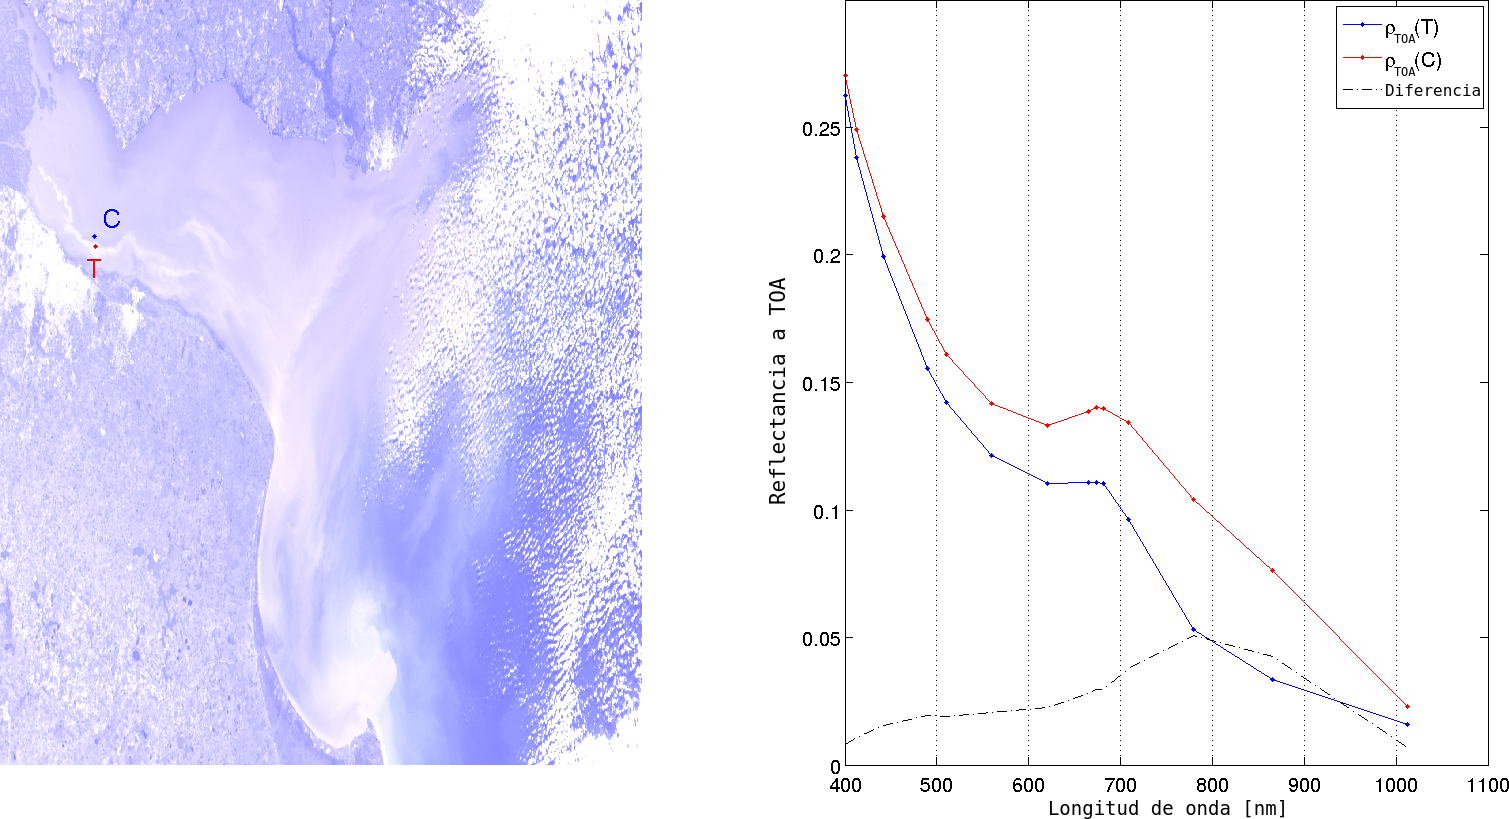
\includegraphics[width=\textwidth]{int/figures/RDP_TC_comparison_B_RHO.png}
    \caption[Reflectancia a TOA de la imagen de OLCI-A del 08-06-2016 sobre el RdP.]{Reflectancia a TOA ($\rho_{TOA}$, Ec. \ref{int:eq:rhotoa}) de la imagen de OLCI-A del 8 de junio de 2016 sobre el RdP. Izq.: Composición RGB - en geometría de sensor - observándose una fuerte componente azul proveniente de la dispersión Rayleigh. Der.: Reflectancias espectrales correspondientes a dos pines dentro de la imagen: \textit{T} (en aguas turbias del RdP) y \textit{C} (en aguas claras).}
    \label{int:RDP_TC_comparison_B_RHO}
    \end{figure}

    \begin{figure}
    \centering
    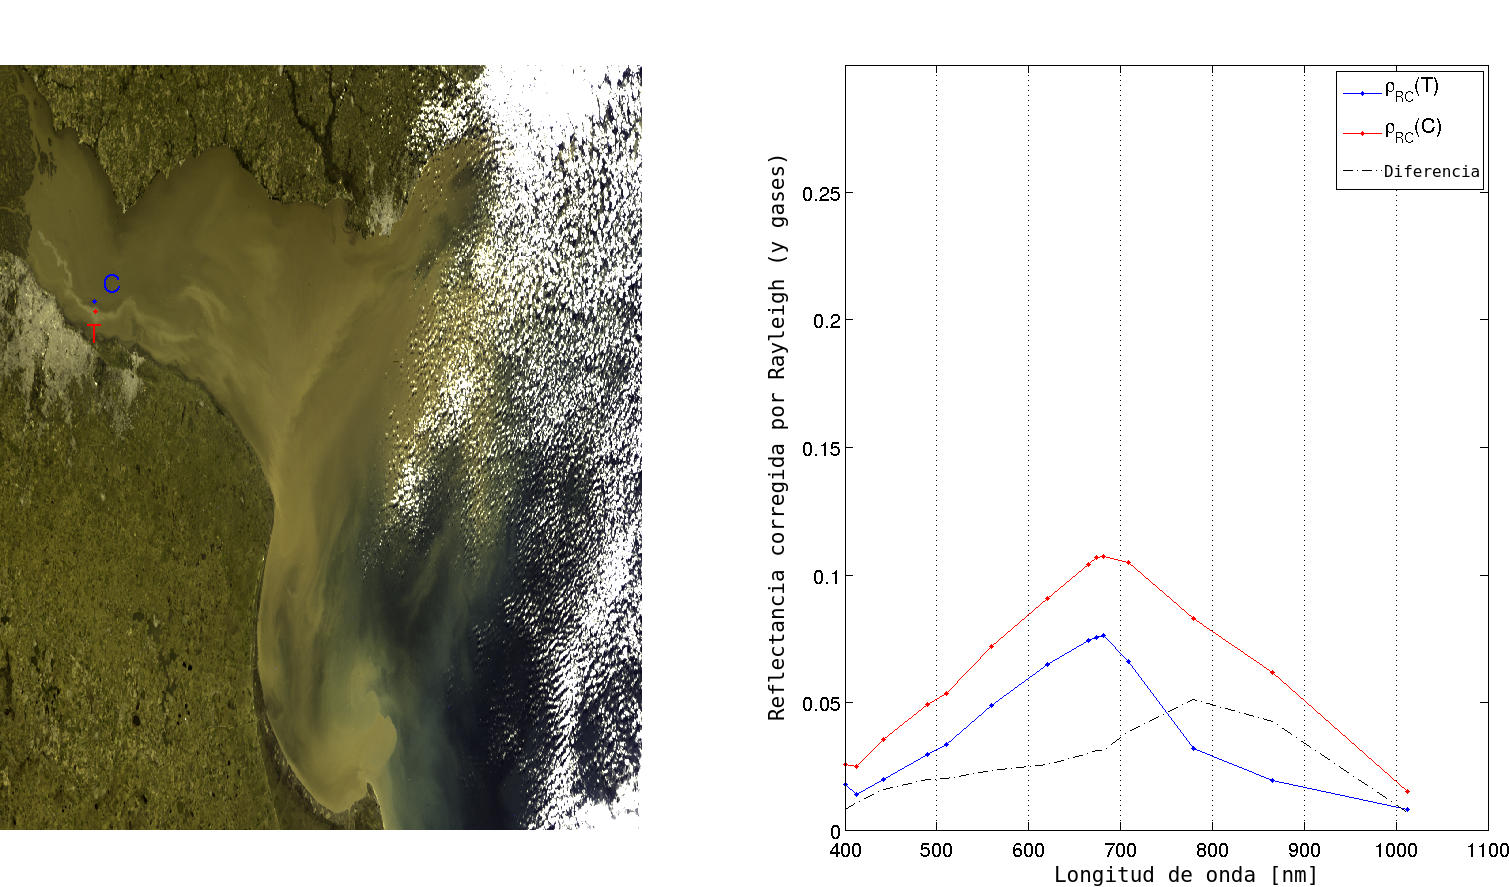
\includegraphics[width=\textwidth]{int/figures/RDP_TC_comparison_B_RHOGRC.png}
    \caption[Reflectancia RC de la imagen de OLCI-A del 08-06-2016 sobre el RdP.]{Ídem Fig. \ref{int:RDP_TC_comparison_B_RHO}, pero para reflectancia corregida por Rayleigh y por absorción de gases.}
    \label{int:RDP_TC_comparison_B_RHOGRC}
    \end{figure}

\section{Dispersión/absorción por Aerosoles (C)}
\label{int:s:aerosoles}

    Los aerosoles son partículas sólidas o líquidas que se hallan en la atmósfera, con tamaños característicos mucho mayores que las moléculas de gas - por lo cual sus propiedades dispersivas se enmarcan dentro del régimen de Mie (Figura \ref{int:scatteringTypes}) - pero a la vez lo suficientemente chicos como para mantenerse suspendidos en la atmósfera por períodos de horas, días o más \cite{mobley2016}. Los radios típicos varían dentro del rango $[0.1 - 10.0] \mu m$. Las propiedades ópticas de aerosoles son determinadas por su composición, la cual se parametriza usualmente a través de su índice de refracción (complejo) y su granulometría (o PSD, por \textit{Particle Size Distribution}). Para el propósito de la CA de imágenes de color es usual utilizar modelos de aerosoles (como los de Shettle y Fenn 1979, \cite{shettle1979}, los de la WMO, \cite{wmo1986} o los utilizados por la NASA de Ahmad et al. 2010, \cite{ahmad2010}) cuyas granulometrías resultan de la suma de dos modos: un modo \textit{fino} (de radios típicos del orden de $1 \mu m$) y uno \textit{grueso} (de radios mayores a $1 \mu m$). A su vez, es conocido que la granulometría de cada uno de estos modos sigue - en la gran mayoría de los casos - una distribución log-normal, por lo que, la distribución cumulativa en volumen resulta, teniendo en cuenta sendos modos: \cite{ahmad2010}
    
    \begin{equation}
        \frac{dV(r)}{d(lnr)} = \sum_{i=1}^{2}\frac{V_{0i}}{\sqrt{2\pi}\sigma_{i}}exp\left[-\left(\frac{ln(r)-ln(r_{v0i})}{\sqrt{2}ln(\sigma_{i})}\right)^{2}\right]
        \label{int:eq:aer_psd}
    \end{equation}
    
    \noindent donde $V(r)$ es el volumen total ocupado por las partículas con radio $r$, típicamente expresado en unidades de $\mu m^{3}cm^{-3}$; $r_{voi}$ y $\sigma_{i}$ son la media geométrica y el desvío estándar del radio del $i-$ésimo modo, respectivamente. Generalmente, el modo fino es de origen continental mientras que el grueso proviene de sales oceánicas.
    
    Las propiedades físicas de los aerosoles determinan sus propiedades ópticas: coeficientes de \textit{absorción} (\S \ref{qssa:s:a}),  \textit{dispersión} (\S \ref{qssa:s:b}) y \textit{función de fase} (\S \ref{sos:s:matrizdefase}). Típicamente - aunque no en todos los casos - es posible representar a los aerosoles como esferas homogéneas, lo que posibilita computar su impacto en el balance radiativo a partir de la Teoría de Mie, \cite{mishchenko2002}. Una vez que los coeficientes de absorción y dispersión específicos - $a^{*}(\lambda)$ y $b^{*}(\lambda)$ - y el perfil de concentraciones - $Conc(z)$ - de los aerosoles son conocidos, es posible computar el coeficiente de \textit{extinción}, $c(z,\lambda) = Conc(z)[a^{*}(\lambda) + b^{*}(\lambda)]$, \S \ref{qssa:s:c}. Luego, siguiendo lo expuesto en \S \ref{sos:s:bouguerlambertbeer}, es posible computar el espesor óptico de aerosoles:
    
    \begin{equation}
        \tau_{a}(\lambda) = \int_{z_{0}}^{TOA}c(z,\lambda) dz
        \label{int:eq:tau_aer_def}
    \end{equation}

    \noindent siendo $z_{0}$ la elevación de la interfase aire-agua (típicamente $z_{0}=0$ km para el Río de la Plata). Esto quiere decir que el espesor óptico de aerosoles en una determinada longitud de onda de referencia es proporcional a la concentración total de aerosoles. Luego, para extrapolar a otras longitudes de onda, es válido, dentro de un rango espectral suficientemente corto, utilizar una ley exponencial:
    
    \begin{equation}
        \tau_{a}(\lambda) = \tau_{a}(\lambda_{0})e^{-c_{\tau}(\lambda-\lambda_{0})}
        \label{int:eq:tau_aer_ang}
    \end{equation}

    \noindent donde $c_{\tau}$ es el coeficiente de decaimiento exponencial, o bien una ley de tipo Angstrom:
    
    \begin{equation}
        \tau_{a}(\lambda) = \tau_{a}(\lambda_{0})\left(\frac{\lambda_{0}}{\lambda}\right)^{\alpha_{\tau}}
        \label{int:eq:tau_aer_exp}
    \end{equation}

    \noindent donde $\alpha_{\tau}$ es el coeficiente de Angstrom. En general, aerosoles más pequeños (grandes) poseen coeficientes de Angstrom más grandes (pequeños), aproximándose al valor de $4$ en el límite de dispersión Rayleigh, Ec. \ref{int:eq:taur}.
    
    \subsection{Escenarios de aerosoles de la WMO}
    \label{int:s:wmo}
        Si bien existen varios catálogos de escenarios de aerosoles, nosotros describiremos muy brevemente los escenarios propuestos por la WMO, \cite{wmo1986}, dado que son los que están incluidos dentro del código de transferencia radiativa CNES-SOS utilizado en esta tesis (\S \ref{sos}). Los escenarios puros cuyos modos son log-normales son tres: el \textit{continental} (WMO-C), el \textit{marítimo} (WMO-M) y el \textit{urbano} (WMO-U) (Cuadro \ref{int:tab:wmo_CMU}). A su vez, cada uno de estos escenarios está conformado por distintas fracciones relativas de los modos de aerosoles de granulometría log-normal, a saber: \textit{polvos}, \textit{hidrosolubles}, \textit{oceánicos} y \textit{hollines} (Cuadro \ref{int:tab:wmo_modos}). 
        
        \begin{table}
        \caption[Proporción de cada componente de aerosoles según escenarios WMO.]{Proporción de cada componente de aerosoles según escenario propuesto por la WMO, \cite{wmo1986}.}
        \begin{tabular}{|l|l|l|l|l|}
        \hline
        \textbf{Escenario WMO} & \textbf{Polvo} & \textbf{Hidrosoluble} & \textbf{Oceánico} & \textbf{Hollín} \\ \hline
        \textbf{Continental}   & 70\%           & 29\%                  & 0\%               & 1\%             \\ \hline
        \textbf{Marítimo}      & 0\%            & 5\%                   & 95\%              & 0\%             \\ \hline
        \textbf{Urbano}        & 17\%           & 61\%                  & 0\%               & 22\%            \\ \hline
        \end{tabular}
        \label{int:tab:wmo_CMU}
        \end{table}

        \begin{table}
        \caption[Parámetros de las granulometrías de los modos log-normalres de aerosoles según reporte de la WMO.]{Parámetros de las granulometrías de los modos log-normalres de aerosoles según reporte de la WMO, \cite{wmo1986}.}
        \begin{tabular}{|l|l|l|}
        \hline
        \textbf{Tipo}         & \textbf{Radio medio [$\mu m$]} & \textbf{Desvío estándar [$\mu m$]} \\ \hline
        \textbf{Polvo}        & 0.5000                         & 2.99                               \\ \hline
        \textbf{Hidrosoluble} & 0.0050                         & 2.99                               \\ \hline
        \textbf{Oceánico}     & 0.3000                         & 2.51                               \\ \hline
        \textbf{Hollín}       & 0.0118                         & 2.00                               \\ \hline
        \end{tabular}
        \label{int:tab:wmo_modos}
        \end{table}

        \begin{figure}
        \centering
        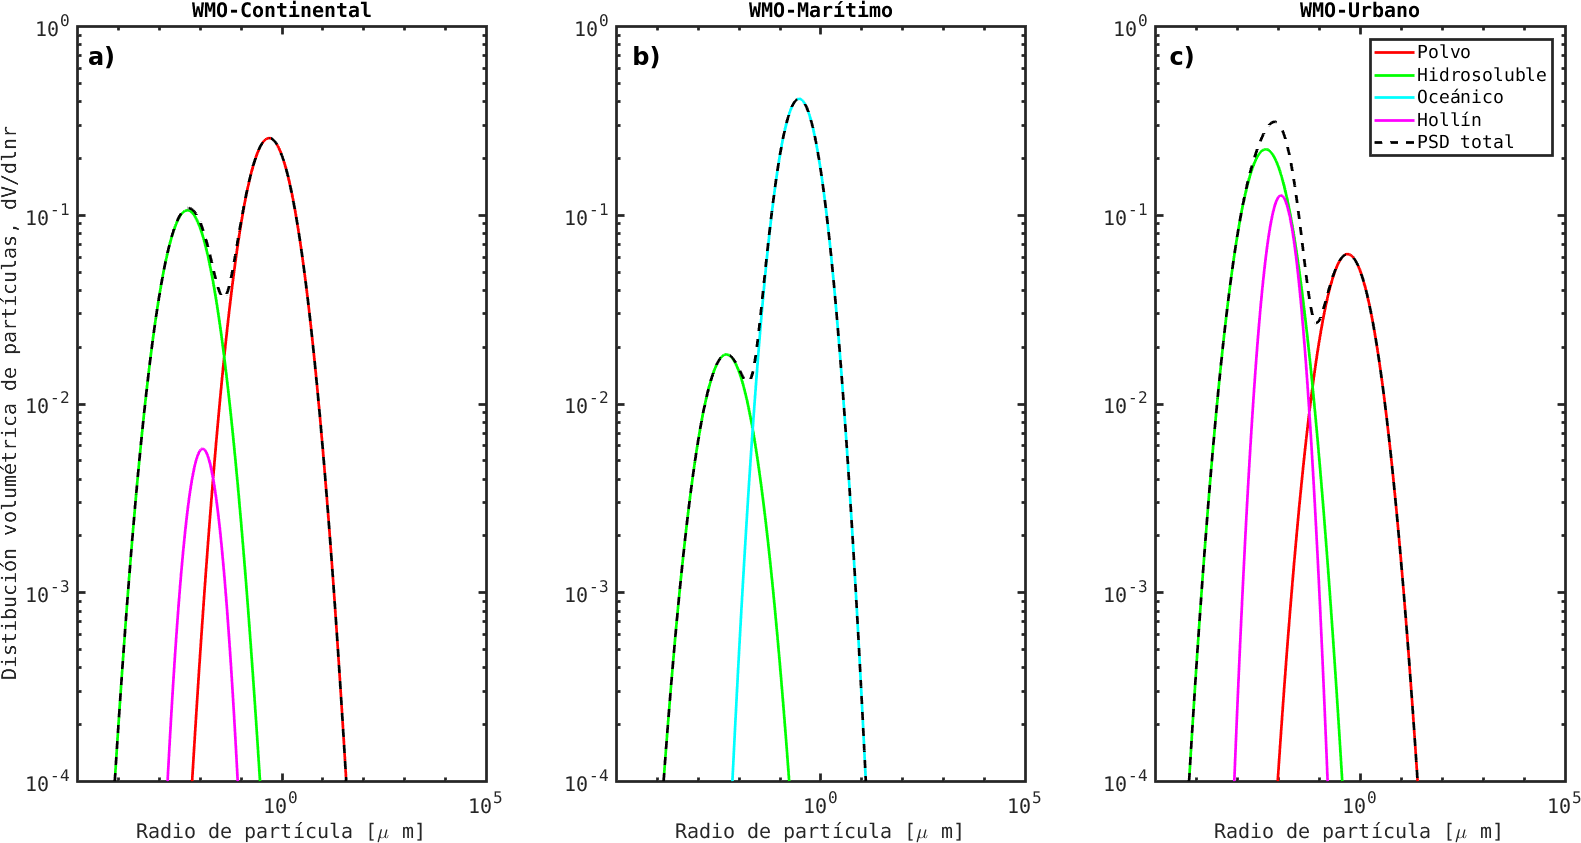
\includegraphics[width=\textwidth]{int/figures/WMO_PSD.png}
        \caption[Distibuciones granulométricas de los escenarios de la WMO.]{Distibución granulométrica, $dV/d(ln(r))$ (Ec. \ref{int:eq:aer_psd}), de los escenarios continental (a), marítimo (b) y urbano (c) propuestos por la WMO, \cite{wmo1986}.}
        \label{int:WMO_PSD}
        \end{figure}
        
        La información detallada de las propiedades de dichos modos de aerosoles (índice de refracción, albedo de dispersión simple, etc.) puede hallarse en \cite{wmo1986} y \cite{lafrance2002}.
    
    \subsection{Estrategias de cómputo de la reflectancia de aerosoles}
	\label{int:s:aer_estrategias}
    
        Contrario al caso de las moléculas de aire, los aerosoles son fuertemente variables en tamaño y composición, por lo que el cómputo de sus propiedades ópticas es más complejo que en el caso de la corrección por dispersión Rayleigh. Existen múltiples estrategias de corrección de aerosoles que podrán ser aplicables o no según el tipo de agua, atmósfera y sensor, de las cuales mencionaremos las principales \textit{familias}.
    
    	\subsubsection{Supuesto de agua negra en el NIR}
    	\label{int:s:ACblackPixelNIR}
    
            Dicho esquema fue desarrollado por Howard Gordon, \cite{gordon1978}\cite{gordon1980}\cite{viollier1980}\cite{gordon1981}\cite{gordon1987}\cite{gordon1988} culminando en el trabajo de Gordon y Wang 1994, \cite{gordon1994}, el cual plantea su aplicabilidad a imágenes SeaWIFS (que portaba dos bandas en el NIR centradas en $765$ nm y $865$ nm). El supuesto de agua negra se basa en el hecho de que la reflectancia proveniente del agua en la región del infrarrojo cercano (NIR) es prácticamente nula (véase Figura \ref{int:casoIyII}). Dicho fenómeno se debe principalmente a la fuerte absorción del agua líquida en dicha región del espectro, \cite{pope1997}\cite{kou1993}.

            Para entender cómo se aplica este supuesto, consideremos la \textit{reflectancia corregida por Rayleigh}, $\rho_{RC}$, que surge tras la corrección por absorción gaseosa, Rayleigh, \textit{sunglint} y \textit{whitecaps}:
            
            \begin{equation}
                \rho_{RC}:=\frac{\rho_{TOA}}{t_{g}}-\rho_{r}-T\rho_{g}-t\rho_{wc} = \rho_{a} + t\rho_{w}
                \label{int:eq:rhoResGW94}
            \end{equation}
            
            \noindent donde hemos expresado los términos de aerosoles como $\rho_{a}$ en vez de $[\rho_{a}+\rho_{ra}]$ por simplicidad. Si asumimos el supuesto de agua negra como válido podremos establecer que, dadas dos bandas en el NIR, $\lambda_{1}$ y $\lambda_{2}$:

            \begin{equation}
                \rho_{RC}(\lambda_{1,2}) \underbrace{=}_{\rho_{w}(\lambda_{1,2})=0} \rho_{a}(\lambda_{1,2})
                \label{int:eq:blackPixelAmplitud}
            \end{equation}

            \begin{equation}
                \epsilon(\lambda_{1},\lambda_{2}):=\frac{\rho_{RC}(\lambda_{1})}{\rho_{RC}(\lambda_{2})} \underbrace{=}_{\rho_{w}(\lambda_{1})=\rho_{w}(\lambda_{2})=0} \frac{\rho_{a}(\lambda_{1})}{\rho_{a}(\lambda_{2})}
                \label{int:eq:blackPixelEpsilon}
            \end{equation}
            
            De esta forma, con poseer al menos dos bandas donde el supuesto de agua negra sea válido es suficiente para establecer una amplitud y un parámetro de variabilidad espectral (tal como $c$ en la Ec. \ref{int:eq:tau_aer_exp} o $\alpha$ en Ec. \ref{int:eq:tau_aer_ang}) para la reflectancia de aerosoles. Luego, mediante la elaboración de LUTs de aerosoles, es posible extrapolar al resto de las bandas la señal de aerosoles determinada en las Ecs. \ref{int:eq:blackPixelAmplitud} y \ref{int:eq:blackPixelEpsilon}. Esto se hace eligiendo modelos de aerosoles - dentro de los que conforman las LUTs - cuyas características espectrales sean coincidentes con las de la reflectancia residual, $\rho_{RC}(NIR)$. Los pasos específicos de cómo es aplicado este esquema por el \textit{software} SeaDAS de la NASA a imágenes MODIS, SeaWIFS, VIIRS, etc. se hallan didácticamente detallados en Mobley et al. 2016, \cite{mobley2016}.

            Dicho esquema tiene dos contras fundamentales:
            
            \begin{enumerate}
                \item No es válido en aguas ópticamente complejas como las del RdP ya que el supuesto de agua negra no es válido en el NIR debido a la elevada retrodispersión de las partículas en suspensión. De hecho, este esquema será únicamente válido en aquellos escenarios donde las concentraciones de fitoplancton y sedimentos sean muy bajas. Afortunadamente, gran parte de las regiones oligotróficas de los océanos cumple dicha condición. En la Figura \ref{int:casoIyII} se muestran valores medidos de reflectacias del agua en escenarios muy contrastantes: el Río de la Plata - donde la reflectancia en el NIR es claramente no nula - y el Golfo San Matías - donde la reflectancia en NIR suele ser cercana a cero o nula.

                \begin{figure}
                \centering
                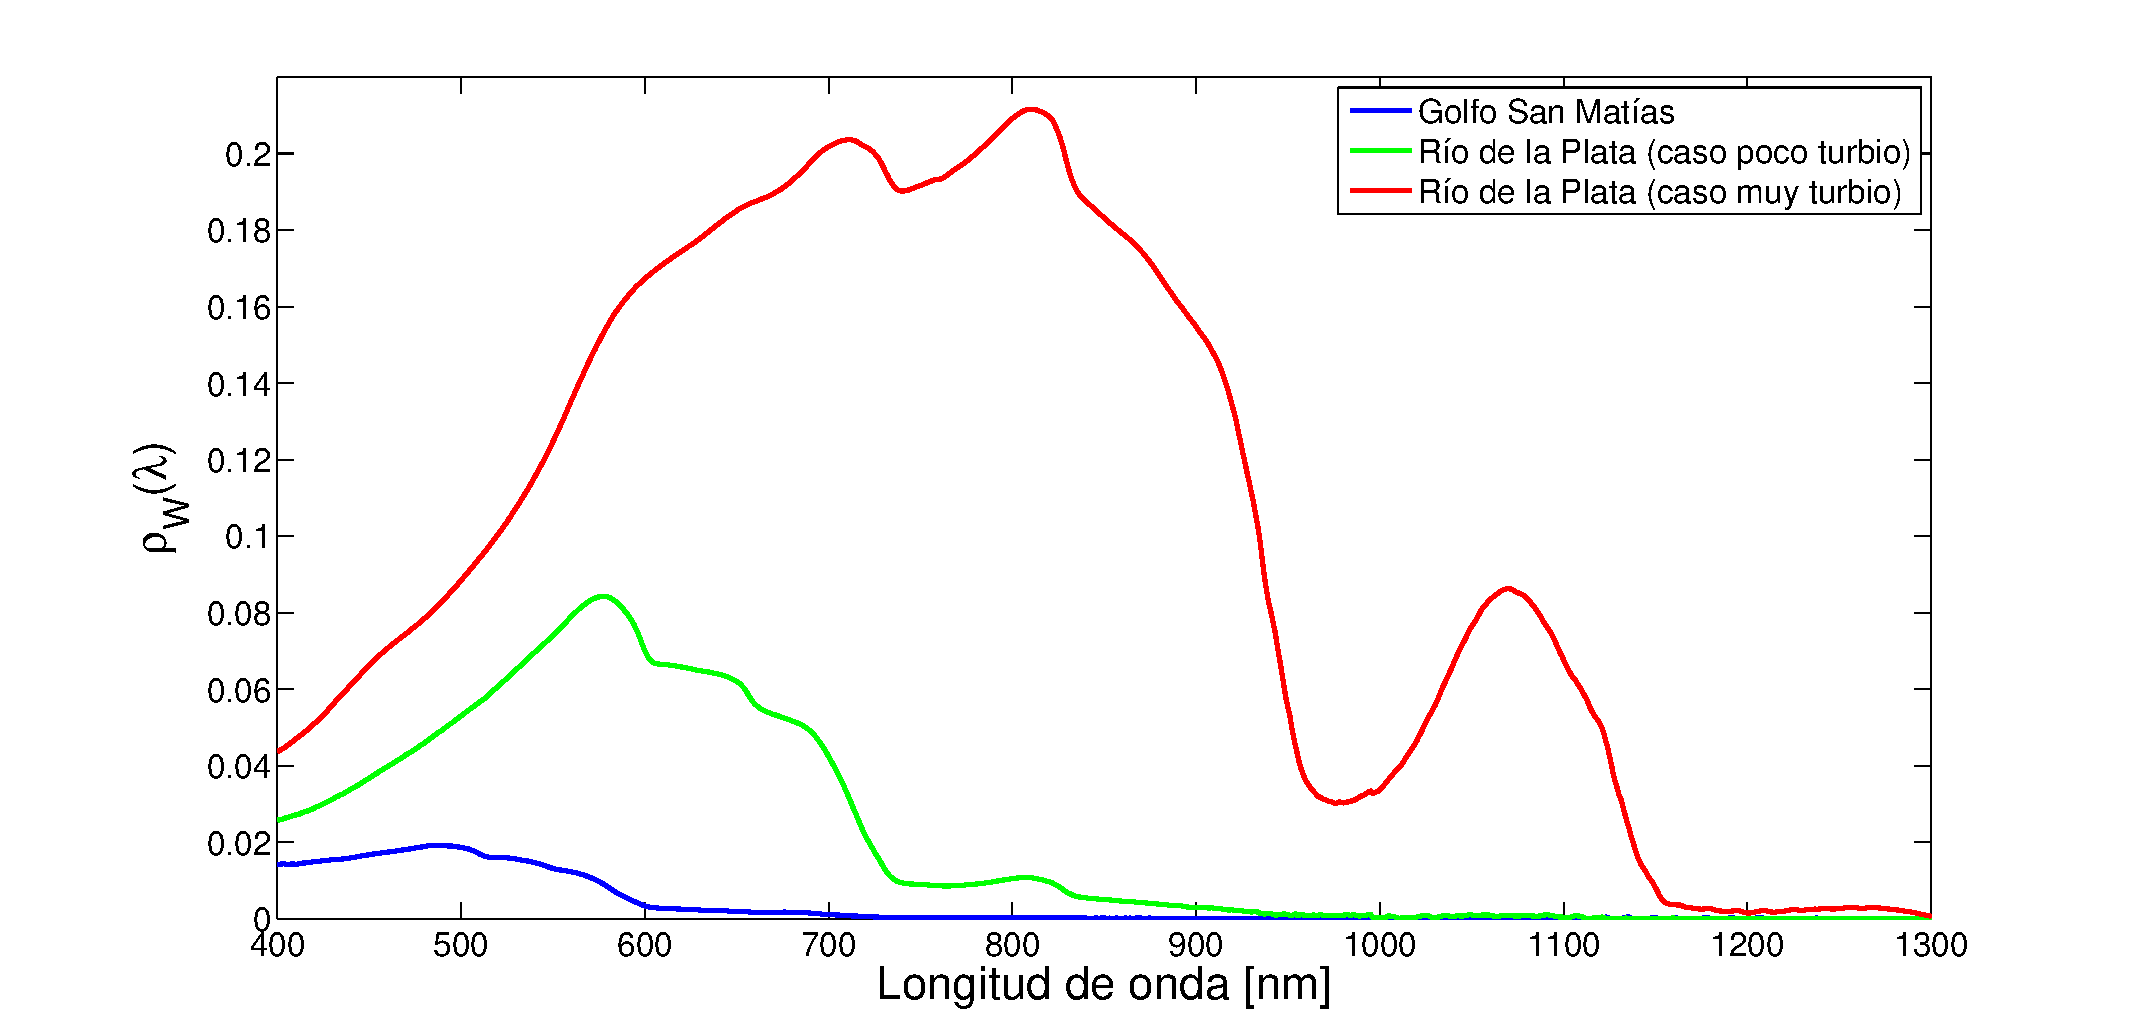
\includegraphics[width=1\textwidth]{int/figures/casoIyII}
                \captionof{figure}[Reflectancias de aguas claras y ópticamente complejas]{Reflectancias medidas sobre cuerpos de agua con características espectrales muy diferentes: el Río de la Plata, donde el supuesto $\rho_{w}(NIR)=0$ es generalmente inválido, y el Golfo San Matías, donde generalmente dicho supuesto es válido. Reflectancia del Golfo de San Matías: cortesía de Gabriela Williams (CENPAT/CONICET).}
                \label{int:casoIyII}
                \end{figure}

                \item Los errores de extrapolación son muy pronunciados en las bandas espectralmente alejadas al NIR: el violeta y el azul. Esto implica que un pequeño error en la determinación de la amplitud o $\epsilon(\lambda_{1},\lambda_{2})$ puede producir grandes errores en la magnitud de $\rho_{a}$ en el azul. A su vez, si consideramos aerosoles fuertemente absorbentes, la extrapolación al azul muchas veces no es biyectiva. Esto quiere decir que al mismo valor de $\epsilon(\lambda_{1},\lambda_{2})$ en el NIR pueden corresponder dos modelos de aerosoles con valores muy disímiles de $\rho_{a}$ en el azul. Es por esto que típicamente no se consideran modelos de aerosoles muy absorbentes en las LUTs utilizadas para dicho esquema de corrección. 
            \end{enumerate}

    	\subsubsection{Esquemas iterativos en el NIR}
    	\label{int:s:ACiterNIR}
    	    La familia de CAs que sucedieron a la de Gordon y Wang 1994, \cite{gordon1994}, plantean esquemas iterativos para poder determinar la señal - no nula - del agua en el NIR. El método perteneciente a esta familia que actualmente es implementado por el OBPG (\textit{Ocean Biology Processing Group}) es descrito en Bailey et al. 2010, \cite{bailey2010}, aunque fue propuesto originalmente por Siegel et al. 2000, \cite{siegel2000}, Stumpf et al. 2003, \cite{stumpf2003}.
    	    
    	    El esquema parte de una corrida inicial en la que se aplica el esquema de agua negra y se obtiene una reflectancia del agua inicial en las bandas del visible (VIS). Luego, a partir de esta reflectancia y utilizando un modelo bio-óptico, se calcula la reflectancia del agua en el NIR y se la sustrae a la señal residual, $\rho_{RC}(NIR)$. De esta forma, se asume que en este primer paso la reflectancia residual se ha aproximado a la condición de agua negra, Ecs. \ref{int:eq:blackPixelAmplitud} y \ref{int:eq:blackPixelEpsilon}. Luego se vuelve a aplicar el procedimiento para obtener una nueva reflectancia del agua en el VIS y en el NIR. Estos pasos se repiten típicamente hasta la convergencia de la estimación o hasta alcanzar un número de iteraciones máximo.
    	    
            Dicho esquema es muy efectivo en escenarios de aguas moderadamente turbias, pero es fuertemente dependiente de la plausibilidad del modelo bio-óptico utilizado para el cálculo de la reflectancia en el NIR. A su vez, la señal del agua es muchas veces lo suficientemente elevada como para saturar las bandas NIR de los sensores, \cite{dogliotti2011}. Existen varias variantes que se basan en esquemas iterativos en el NIR: por ejemplo, el esquema modificado de Wang et al. 2012, \cite{wang2012}, utilizado para GOCI (Geostationary Ocean Color Imager), o el esquema BPC (\textit{Bright Pixel Correction}) aplicado sobre OLCI, \cite{moore1999}\cite{moore2011}\cite{moore2017}\cite{lavender2005}, aunque esta última no depende de un modelo bio-óptico en el VIS.

    	\subsubsection{Supuesto de agua negra en el SWIR}
    	\label{int:s:ACswir}
    
            La generación de sensores que fue lanzada al espacio tras el SeaWIFS, (por ej. MODIS, VIIRS, OLI, MSI), tiene incoporadas aparte de las bandas en el VIS y el NIR, bandas en el SWIR lejano $[1200 - 2500]$ nm, donde la absorción del agua líquida es varias veces mayor que en el NIR. Esto implica que el supuesto de agua negra sigue siendo válido en esta región del espectro; aunque para el caso extremo del frente de turbidez del Río de la Plata, esta hipótesis comienza a vulnerarse también en la banda del SWIR centrada en $1240$ nm, \cite{knaeps2012}, por lo que este cuerpo de agua resulta un desafío aún mayor a la hora de aplicar una CA basada en las bandas del SWIR.

            El esquema de agua negra en el SWIR fue propuesto por Wang y Shi 2005, \cite{wang2005} y se resume a continuación:

            \begin{enumerate}
                \item Los valores de $\rho_{RC}(SWIR)$ son utilizados de manera equivalente que los casos de aguas claras, asumiendo agua negra en el SWIR, para obtener un modelo de aerosoles extrapolable a las bandas del NIR.
                \item Luego se obtienen, a partir de dicho modelo de aerosoles, los valores de $\rho_{w}(NIR)$.
                \item Finalmente, sustrayendo estos valores de $\rho_{w}(NIR)$ a $\rho_{RC}(NIR)$, el esquema se halla en las condiciones iniciales correspondiente a aguas claras, por lo que se puede proceder a la extrapolación desde el NIR hacia el VIS.
            \end{enumerate}
            
            La problemática esencial que tienen las bandas del SWIR es que su razón señal-ruido (SNR) suele ser menor que la SNR de las bandas NIR, sumado al hecho de que son espectralmente más distantes a las bandas del VIS. Esto implica que la extrapolación mediante LUTs posea aún mayores inconvenientes que en el caso anterior. Aparte, no todos los sensores poseen bandas en el SWIR lejano debido a su elevado costo (por ej. OLCI y MERIS).

    	\subsubsection{Algoritmo NIR-SWIR}
    	\label{int:s:ACnirswir}
    	    El algoritmo NIR-SWIR fue desarrollado por Wang y Shi 2007, \cite{wang2007} y en realidad resulta en la aplicación del algoritmo NIR o SWIR dependiendo del grado de turbidez del agua, determinado por un índice propuesto por Shi y Wang 2007, \cite{shi2007}. En caso de que dicho índice exceda un umbral de turbidez mínimo, se aplica el esquema SWIR, \S \ref{int:s:ACswir}; caso contrario, se procede al esquema NIR iterativo de Bayley et al. 2010, \S \ref{int:s:ACiterNIR}. Si bien dicho algoritmo es aplicable a muchos cuerpos de agua, posee todos los defectos combinados de los dos esquemas en los que se basa. A su vez, el índice de turbidez en el que se basa suele no ser plausible en aguas turbias como las del RdP.

        \subsubsection{Supuesto de homogeneidad espacial}
        \label{int:s:ACmumm}
            Esta familia de algoritmos se basa en la idea originalmente descrita en Ruddick et al. 2000, \cite{ruddick2000}. A continuación, haremos una breve descripción del esquema:
            
            \begin{enumerate}

                \item Habiendo determinado la reflectancia residual o corregida por Rayleigh, notamos que se tiene:
                \begin{equation}
                    \rho_{RC}(\lambda_{i})=\rho_{a}^{I}(\lambda_{i})+t^{I}(\lambda_{i})\rho_{w}(\lambda_{i})\quad \forall i=1,...,N
                    \label{int:eq:RUDD:rhoCORR}
                \end{equation}
                
                \noindent siendo $I$ el modelo de aerosoles a determinar, $i$ el número de banda del sensor y $N$ el número total de bandas de interés. Se asumirá por simplicidad que el sensor en cuestión es el SeaWIFS; por lo que $N=8$; las bandas corresponden al visible para $1<i<6$, mientras que $i=7,8$ son bandas en el NIR ($765$ nm y $865$ nm).
                
                \item También se conoce, una vez determinado el modelo de aerosoles $I$, el parámetro espectral $\epsilon$:
                \begin{equation}
                \epsilon(\lambda_{i},\lambda_{j})=\frac{g^{I}(\rho_{a}^{I}(\lambda_{i}))}{g^{I}(\rho_{a}^{I}(\lambda_{j}))}
                \label{int:eq:RUDD:epsilon}
                \end{equation}
    
                \noindent siendo $g^{I}$ la transformación casi-lineal que lleva $\rho_{a}^{I}$ a $\rho_{a,s}^{I}$.
                
                \item Esto implica un total de 15 ecuaciones (las 8 de la Ec. \ref{int:eq:RUDD:rhoCORR} y las 7 de la Ec. \ref{int:eq:RUDD:epsilon}) para 17 incógnitas (los 8 valores de $\rho_{a}$, los 8 valores de $\rho_{w}$ y el modelo de aerosoles a determinar, $I$). En el esquema de agua negra en el NIR, el sistema se cerraba con dos condiciones más, $\rho_{w}(\lambda_{i})=0\quad i=7,8$.

                \item En el trabajo de Ruddick et al. 2000 \cite{ruddick2000} se propone la \textit{hipótesis de homogeneidad espacial en la región del NIR}. La misma asume los parámetros $\alpha_{7,8}$ y $\epsilon_{7,8}$ como valores fijos en una región acotada alrededor de determinado píxel en la imagen, siendo
                            
                \begin{equation}
                    \begin{aligned}
                        \epsilon_{7,8}&=\frac{\rho_{a}(\lambda_{7})}{\rho_{a}(\lambda_{8})}\\
                        \alpha_{7,8}&=\frac{\rho_{w}(\lambda_{7})t(\lambda_{7})}{\rho_{w}(\lambda_{8})t(\lambda_{8})}
                        \label{int:eq:RUDD:alphaydelta}
                    \end{aligned}
                \end{equation}
                    
                Dichos valores pueden ser obtenidos por procesos de calibración de la región de la imagen (véase \cite{ruddick2000}) donde se asume válida la hipótesis de homogeneidad.
            \end{enumerate}
            
            El mayor problema de este método reside en el hecho de que, en muchas ocasiones, la asunción de homogeneidad espacial no es válida o bien es difícil estimar el rango espacial de validez. Aparte, el requerimiento de computar los valores de los parámetros $\alpha_{7,8}$ y $\delta_{7,8}$ para múltiples regiones reducidas de una imagen implica un agregado al costo computacional e imposibilitando la automatización del proceso.

        \subsubsection{Supuesto de agua negra en el UV}
        \label{int:s:ACUV}
            Dicho supuesto fue planteado por primera vez por He et al. 2012, \cite{he2012}, y es en principio aplicable en aguas con elevado contenido de detrito orgánico y partículas no algales en suspensión, donde la elevada absorción del dichas sustancias hace que la reflectancia del agua en el UV se aproxime a 0, $\rho_{w}(UV)=0$, de forma tal de que la reflectancia RC en dichas bandas permite mejorar la calidad de la extrapolación al VIS a partir de la información provista por las bandas NIR y/o SWIR.
            
            El problema de dicho esquema es la mayoría de los sensores remotos vigentes no poseen bandas en el UV, más allá de que las mismas suelen presentar problemas de calibración y ruido. A su vez, el supuesto es únicamente válido en escenarios turbios. Si bien se ha esbozado la hiótesis de que el supuesto del NIR podría eventualmente extenderse al violeta asumiendo un valor constante de reflectancia, $\rho_{w}(400 nm)=cte>0$ (supuesto de \textit{anclaje} en el violeta), dicha hipótesis no ha sido demostrada hasta el momento.

        \subsubsection{Esquemas acoplados de espectro completo}
        \label{int:s:ACacoplados}
            Existen varios algoritmos que utilizan toda la información espectral disponible para realizar la CA, distinto de los previamente mencionados - que únicamente utilizan algunas bandas posicionadas en regiones estratégicas del espectro. Los mismos utilizan modelos acoplados de las propiedades ópticas de la atmósfera y el agua basados en una optimización o un enfoque iterativo para obtener una combinación más adecuada de pares de reflectancias agua-aerosoles, como por ejemplo en Doerffer y Schiller 2007, \cite{doerffer2007}, Chomko y Gordon 2001, \cite{chomko2001}. Dichos enfoques incluso han logrado la remoción exitosa del \textit{sunglint}, señal intensa pero espectralmente simple (por ejemplo, POLYMER, Steinmetz et al. 2011, \cite{steinmetz2011}) y tienden a proporcionar espectros plausibles de reflectancia de agua, evitando - por condiciones de contorno preestablecidas - reflectancias negativas. Incluso han demostrando ser muy robustos para datos con sesgos de calibración. Entre estos esquemas también podríamos incluir las inversiones basadas en redes neuronales, como en el caso de Jamet et. al 2005, \cite{jamet2005}, o bien las basadas en inferencia bayesiana, como el algoritmo desarrollado en Frouin y Pelletier 2015, \cite{frouin2015}.
            
            A pesar del éxito de estos algoritmos en varias circunstancias, los mismos se respaldan en modelos ópticos tanto de la atmósfera como del agua demasiado simples y que muchas veces no son representativos de la realidad. Por otro lado, dada la complejidad subyacente, en caso de no producir buenos resultados, es difícil hallar el origen de la falla en la estimación en comparación con los esquemas extrapolativos clásicos.

\section{Transmitancia directa (D)}
\label{int:s:tDir}

    Dicha transmitancia se aplica a términos de superficie que puedan ser considerados especulares, como el caso del \textit{sunglint}, donde el camino recorrido por los fotones interactuantes con la superficie es aproximadamente proporcional al factor de masa de aire (Ec. \ref{int:eq:mu}) al igual que en el caso de absorción de gases estratosféricos. De esta forma, aplicando la Ley de Bouguer-Lambert-Beer, \S \ref{sos:s:bouguerlambertbeer}, obtenemos la siguiente expresión:
    
    \begin{equation}
        T = T_{s}T_{v} = e^{-\tau/cos(\theta_{s})}e^{-\tau/cos(\theta_{v})} = e^{-\tau \mu}
        \label{int:eq:tDir}
    \end{equation}
    
    \noindent donde $\tau$ es el espesor óptico total de la atmósfera debido a procesos dispersivos. Considerando a las moléculas de aire y los aerosoles, resulta entonces $T = e^{-(\tau_{r} + \tau_{a})\mu}$.
    
\section{Reflexión especular del sol o \textit{sunglint} (E)}
\label{int:s:sunglint}
    
    Dado que el índice de refracción relativo de la interfase agua-aire es prácticamente constante a lo largo del UV-VIS-NIR-SWIR ($n\approx 1.334$), y el hecho de que las reflectancias de la Ec. \ref{int:eq:rhotoa} están normalizadas por la irradiancia solar, el término de reflectancia de \textit{sunglint} es casi espectralmente constante - a excepción del esperable acople de dicha señal con la atmósfera, modelado por los términos de transmitancia directa y de absorción gaseosa. De hecho, Wang y Bailey 2001, \cite{wang2001}, modelan dicha señal - amén de la transmitancia - como una constante espectral cuya variabilidad angular está dada por la geometría de iluminación y la rugosidad de la interfase agua-aire, a su vez parametrizada por la intensidad del viento en superficie, $w$, siguiendo nuevamente la Ec. \ref{int:eq:coxmunk}:
    
    \begin{equation}
        T(\theta_{v},\theta_{v})\rho_{g} = T(\theta_{v},\theta_{v})c(\theta_{v},\theta_{v},w)
        \label{int:eq:rhoglint}
    \end{equation}
    
    \noindent donde $\partial c/\partial \lambda = 0$. Si bien originalmente el \textit{sunglint} está incluido en las LUTs utilizadas para la corrección Rayleigh, el efecto del mismo es usualmente removido de las mismas y tratado aparte. Aunque en la actualidad existen algoritmos que resuelven la señal del \textit{sunglint} en conjunto con la señal de aerosoles (tales como POLYMER, \cite{steinmetz2011}), en escenarios de \textit{sunglint} extremo la señal de esta componente es tan alta que típicamente los píxeles afectados deben ser enmascarados. Es por esto que en muchos casos los sensores remotos no apuntan directamente al nadir, sino que suelen ser rotados de forma tal de que el \textit{sunglint} no contamine el centro de las imágenes, sino - en los casos de sensores polares heliosincrónicos - únicamente la porción \textit{este} dentro de la franja de barrido, como fue el caso del SeaWiFS.

\section{Transmitancia difusa (F)}
\label{int:s:tDif}

    La tranmitancia difusa es más difícil de modelar que la directa, puesto que se aplica a términos de superficie \textit{aproximadamente} lambertianos ($\rho_{wc}$ y $\rho_{w}$), por lo que el espesor de atmósfera recorrido por la radiación resulta incierto. En esta tesis se utilizará la siguiente expresión, sugerida por Tanre et al. 1979, \cite{tanre1979}:
    
    \begin{equation}
        t = e^{-(\sum_{i}^{N}(1-\frac{b_{b,i}}{b_{i}})\tau_{i})\mu}
        \label{int:eq:tDif0}
    \end{equation}
    
    \noindent donde $b_{i}$, $b_{b,i}$ y $\tau_{i}$ son los coeficientes de dispersión y retrodispersión (Ecs. \ref{qssa:eq:b} y \ref{qssa:eq:bb}) y el espesor óptico debido a la dispersión de la especie $i-$ésima. En nuestro caso, aproximaremos el coeficiente de retrodispersión de los aerosoles como $b_{b,a} = \frac{1}{6}b_{a}$, \cite{tanre1979}, y apelando a la isotropía de la dispersión Rayleigh, la transmitancia difusa resulta

    \begin{equation}
        t = e^{-(\frac{5}{6}\tau_{a} + \frac{1}{2}\tau_{r})\mu}
        \label{int:eq:tDif}
    \end{equation}

    \noindent o bien directamente omitiremos el efecto de los aerosoles en dicha expresión. Para entender este factor en más detalle, véase \cite{mobley2016}.

\section{Reflectancia de espuma o \textit{whitecaps} (G)}
\label{int:s:whitecaps}

    El efecto óptico causado por la espuma en superficie puede ser aproximado por un término lambertiano espectralmente blanco para longitudes de onda menores a 600 nm cuya intensidad variará según la fracción de superficie abarcada por la espuma, $f$. En el procesador estándar de la NASA, dicha fracción se parametriza en función del viento en superficie, $w$, siguiendo a Stamska y Petelski 2003, \cite{stramska2003}:
    
    \begin{equation}
        f = 8.75\times 10^{-5}(w[m/s]-6.33)^3
        \label{int:eq:rhoWC_f}
    \end{equation}

    \noindent mientras que la expresión para la reflectancia de espuma normalizada a $f=1$, $\rho^{*}_{wc}(\lambda)$, proviene de Frouin et al. 1996, \cite{frouin1996}:
    
    \begin{equation}
        \rho^{*}_{wc}(\lambda) = \left\{ \begin{array}{lcc}
                     1 &   si &  \lambda \leq 600 nm \\
                     e^{-0.00175(\lambda-600)} &  si & \lambda > 600 nm\\
                     \end{array}
           \right.
        \label{int:eq:rhoWC_a}
    \end{equation}
    
    En esta tesis, no consideraremos en general el efecto procovado por la espuma, dado que trabajaremos con aguas turbias - es decir, más reflectivas - por lo que podremos despreciar el efecto de la espuma.
\section{Área de estudio}
\label{int:s:area}

    El Río de la Plata (RdP) es uno de los sistemas estuariales más grandes del mundo ($\sim 35000$ km$^{2}$) drenando la segunda cuenca más grande de América del Sur luego del Amazonas. Tiene una longitud de $270$ km y un ancho de más de $220$ km en su boca (Figura \ref{int:rdp}) y sus aguas son poco profundas ($<20$ m). Se estima que la cantidad de sedimentos que transporta varía entre $80$ y $160$ millones de toneladas por año, lo cual lo lleva a ser uno de los ríos más turbios del mundo con valores de SPM de $10$ a $500$ mg/l (\S \ref{dat}). El RdP se caracteriza por la presencia de una zona de máxima turbidez asociada a un frente salino donde se produce el encuentro del agua dulce del río y el agua salada del océano, \cite{guerrero1997}\cite{mianzan2001}. La posición de dicho frente está principalmente controlada por la batimetría coincidiendo su posición media con la Barra del Indio en el sector norte y con la isobata de $5$ m en la Bahía de Samborombón hacia el sur. La gran cantidad de sedimentos transportados por el RdP influye, entre otros, en los procesos sedimentológicos cuyo estudio y comprensión resulta importante para un número de aplicaciones en zonas costeras. Varios estudios respaldados en datos de color del mar se han realizado para determinar el área de influencia de la pluma de agua turbia del Río de la Plata sobre aguas costeras del Atlántico Sudoccidental adyacente al estuario \cite{carvalho2014}\cite{garcia2008}\cite{piola2004}\cite{piola2008}.
    
    \begin{figure}
    \centering
    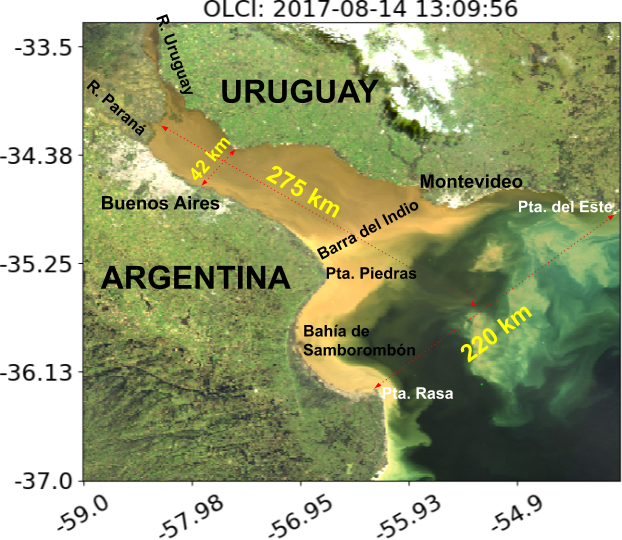
\includegraphics[width=\textwidth]{int/figures/rdp.png}
    \caption[Composición RGB del Río de la Plata.]{Composición RGB de la imagen OLCI del 14-AGO-2017 del Río de la Plata.}
    \label{int:rdp}
    \end{figure}

    Dadas las características particulares del RdP, gran superficie y alto SPM, esta región resulta un gran desafío y un área ideal para evaluar y desarrollar algoritmos de CA que permitan estimar la turbidez o concentración de  material en suspensión a partir de información satelital. En un primer estudio, Dogliotti et al. 2011, \cite{dogliotti2011} analizó en forma cualitativa el desempeño de tres algoritmos de CA aplicados a imágenes MODIS-Aqua en el RdP: i) el algoritmo de CA estándar de la NASA basado en las bandas NIR, \S \ref{int:s:ACiterNIR}; ii) el algoritmo NIR-SWIR, \S \ref{int:s:ACnirswir}, y iii) el algoritmo híbrido propuesto por Wang et al. 2011, \cite{wang2011} entre las estrategias NIR-SWIR y la de homogeneidad espacial, \S \ref{int:s:ACmumm}. Este estudio preliminar mostró - como era esperado - que el supuesto de agua negra en el NIR no se cumple en el RdP debido a la alta concentración de partículas en suspensión. A su vez, muestra que el procedimiento basado en el supuesto de agua negra en el SWIR tampoco genera buenos resultados para imágenes MODIS, puesto que muestra patrones espaciales correlacionados entre las reflectancias del agua y de aerosoles en la zona de máxima turbidez. Por último, si bien muestra buenos resultados para el esquema de Wang et al. 2011, este último posee las falencias propias de los esquemas basados en la homogeneidad espacial. Para otros sensores, como OLCI, se han visto resultados no satisfactorios para el esquema de CA estándar propuesto por la ESA (por lo menos hasta la versión 2.23, \S \ref{blr:s:results:blrac}).
    
    En resumen, estos resultados no concluyentes de las CA preexistentes evidencian la necesidad de realizar un análisis cuantitativo con datos radiométricos de campo y evaluar y/o desarrollar algoritmos alternativos.

\section{Objetivos}
\label{int:s:objetivos}
    La propuesta de tesis planteada propone como objetivo general mejorar la calidad de la información que se obtiene de sensores remotos a bordo de satélites con el fin de mapear la distribución espacio-temporal de variables biogeofísicas, como  la concentración de sedimentos en suspensión, en las aguas dominadas por sedimentos del Río de la Plata. En particular, se pretende llevar a cabo dicho objetivo mediante la exploración de nuevos esquemas de corrección atmosférica que mejoren las estimaciones de la reflectancia del agua en aguas turbias. El trabajo planteado contribuirá en forma directa a la misión argentino-brasileña SABIA-Mar por lo que varias de las simulaciones fueron realizadas para un sistema satélite-sensor con las características del propuesto para dicha misión. Con el fin de alcanzar el objetivo general se plantearon los siguientes objetivos específicos:
    
    \begin{enumerate}
    \item Continuar la colección de datos ópticos de reflectancia en muestras de agua de superficie en el Río de la Plata y organizar sistemáticamente los datos bio-ópticos en una base de datos. 
    \item Desarrollar algoritmos semi-empíricos para derivar la reflectancia del agua usando datos de campo y simulaciones de transferencia radiativa para SABIA-Mar y para diferentes sensores.
    \item Evaluar el desempeño de las correcciones atmosféricas desarrolladas.
    \item Desarrollar aplicaciones y potenciales productos del sensoramiento de color del mar sobre el área del Río de la Plata. 
    \end{enumerate}

\section{Descripción de la estructura de la tesis}
\label{int:s:estructura}

    Esta tesis está escrita en ocho capítulos:
    
    \begin{enumerate}
        \item En el capítulo \ref{int} se introdujeron los conceptos fundamentales de la teledetección del color del mar, de la corrección atmosférica y del área de estudio, con especial énfasis en aquellos que serán requeridos como bagaje previo a los capítulos posteriores.
        \item En el capítulo \ref{dat} se describirán las tareas de campo desarrolladas para calibrar/validar los algoritmos descriptos en los siguientes capítulos, así como un breve análisis de los datos de campo obtenidos. Por último se describirá la estructura de la base de datos confeccionada para sistematizar el almacenamiento y procesamiento de las mediciones realizadas.
        \item En el capítulo \ref{blr} se describirá el algoritmo BLR-AC desarrollado para aguas ópticamente complejas, específicamente para el conjunto de sensores OLCI, que carecen de bandas espectrales en el SWIR lejano, pero que poseen una novedosa banda en el SWIR cercano (1016 nm), que provee de información relevante para el proceso de remoción de aerosoles.
        \item En el capítulo \ref{pca} se describirá el algoritmo SWIR-PCA desarrollado para aguas ópticamente complejas del Río de la Plata para sensores como SABIA-Mar y MODIS que poseen bandas en la región espectral del SWIR lejano, es decir donde es válido el supuesto de agua negra para cualquier concentración de sedimentos.
        \item En el capítulo \ref{ppe} se describirá un procedimiento de corrección de las imágenes de OLCI y MERIS, necesario debido al efecto de eventos de partículas veloces que impactan en los sensores en la región Anomalía Magnética del Atlántico Sur - en particular, afectando las imágenes del Río de la Plata. Dicha corrección forma parte del preprocesamiento realizado previo a la corrección atmosférica descrita en el capítulo \ref{blr}.
        \item En el capítulo \ref{cam} se describirá una aplicación específica al estudio de imágenes de color del mar sobre las aguas ópticamente complejas como las del Río de la Plata: el algoritmo FAIT de detección de vegetación flotante en aguas turbias.
        \item En el capítulo \ref{oil} se describirá otra aplicación específica a estas imágenes: se describirá un posible algoritmo de detección de derrames de hidrocarburos en aguas turbias, junto con diversos índices que permitirían determinar el espesor de la capa superficial del derrame.
        \item En el capítulo \ref{con} se detallarán las conclusiones y las perspectivas a futuro de la presente tesis.
    \end{enumerate}